

\documentclass{article}
\usepackage[utf8]{inputenc}

\usepackage{mathtools, amsmath, amssymb, amstext, amsfonts, mathrsfs, booktabs}
\usepackage[dvipsnames]{xcolor} % to show colorful code
\usepackage{colortbl}
\usepackage{natbib}
\usepackage[nottoc]{tocbibind} % to have the Bibliography listed as a point in the table of contents
\usepackage{graphicx}
\usepackage{blkarray} % to use the blockarray
\usepackage{longtable} % to have tables span more than one page
\usepackage{tikz, xparse} %for the graphs
\usetikzlibrary{shapes, fit,positioning}
\usepackage{subcaption} % to fit two graphs next to each other
\newcommand{\comm}[1]{} % for doing comments longer than one line
\usepackage{listings} % to display the code
\usepackage{color}
\lstset{ %
  language=R,                     % the language of the code
  basicstyle=\footnotesize,       % the size of the fonts that are used for the code
  numbers=left,                   % where to put the line-numbers
  numberstyle=\tiny\color{gray},  % the style that is used for the line-numbers
  stepnumber=1,                   % the step between two line-numbers. If it's 1, each line
                                  % will be numbered
  numbersep=5pt,                  % how far the line-numbers are from the code
  backgroundcolor=\color{white},  % choose the background color. You must add \usepackage{color}
  showspaces=false,               % show spaces adding particular underscores
  showstringspaces=false,         % underline spaces within strings
  showtabs=false,                 % show tabs within strings adding particular underscores
  frame=single,                   % adds a frame around the code
  rulecolor=\color{black},        % if not set, the frame-color may be changed on line-breaks within not-black text (e.g. commens (green here))
  tabsize=2,                      % sets default tabsize to 2 spaces
  captionpos=b,                   % sets the caption-position to bottom
  breaklines=true,                % sets automatic line breaking
  breakatwhitespace=false,        % sets if automatic breaks should only happen at whitespace
  title=\lstname,                 % show the filename of files included with \lstinputlisting;
                                  % also try caption instead of title
  keywordstyle=\color{MidnightBlue},      % keyword style
  commentstyle=\color{darkgray},   % comment style
  stringstyle=\color{PineGreen},      % string literal style
  %escapeinside={\%*}{*)},         % if you want to add a comment within your code
  morekeywords={*,...}            % if you want to add more keywords to the set
} 
\definecolor{darkgray}{gray}{0.25}
\definecolor{gray}{rgb}{0.5,0.5,0.5}
\definecolor{mauve}{rgb}{0.58,0,0.82}

%\pagestyle{headings} %to display headers, the normal way
\usepackage{fancyhdr} % to display headers, the fancy way
\pagestyle{fancy}
\fancyhf{}
\rhead{Schau, Gotzian, Shulman}
\lhead{Evaluating Agarwal et al. 2015}
\rfoot{Page \thepage}

\usepackage{hyperref} % has to be the last package imported
\hypersetup{
    colorlinks=false, % the next lines only work if set to true
    linkcolor=blue,
    filecolor=magenta,      
    urlcolor=cyan,
}

\begin{document}

\begin{titlepage}
    \begin{center}
        
\includegraphics[width=0.4\textwidth]{leuphanalogo}       
        \vspace*{1cm}
        
        \huge
        \textbf{Do organic search results help or
hurt sponsored search
performance?}
        
        \vspace{0.5cm}
        \LARGE
        Evaluating the probabilistic model \\ by Agarwal et al. 2015
        
        \vspace{1.5cm}
        \large
        \textbf{Lisa Gotzian}\\
        \textbf{Erik Schau}\\
        \textbf{Ian Shulman}
        
        \vfill
        \large
        A paper presented for the course \\
        \textbf{Probabilistic Modelling}\\
        instructed by\\
        \textbf{Prof. Dr. Burkhardt Funk}\\
        in the Master's Program\\
        \textbf{Management \& Data Science}
        
        \vspace{0.8cm}
        
        August 26, 2018
        
    \end{center}
\end{titlepage}
\thispagestyle{empty} % to not have a header
\tableofcontents
\newpage
\section{Introduction} \label{sec:intro}
Bayesian hierarchical models have gained quite some importance in the marketing segment during the last 15 years \citep{rossibook, ghose, agarwal_organic_2015}. They are now being employed to analyze click-behavior and orders to evaluate the effectiveness of advertisements in search engines. Eventually, the factors that lead to this behavior are modeled and given a certain importance.\\
Among factors such as sponsored competition, an ad's position relative to other ads, or the quality score of a given keyword, organic search results have not extensively been taken into account. Following the approach of Agarwal et al. 2015., this paper rebuilds and comments on a bayesian hierarchical model that assesses the role of organic search results in particular.\\
The paper is broken up into the following sections: first, a brief overview of the research performed by Agarwal et al in their paper "Do organic search results help or hurt sponsored search performance?" \citep{agarwal_organic_2015}, as well as an explanation of their development, and our interpretation of their model; then, a discussion on the data used for the model, our attempts to simulate the data based on the provided (and some noticeably absent) summary statistics; further, there is an outline of the model estimation made using MCMC sampling and related packages in R; finally, an evaluation of the model describing challenges faced in extrapolating Agarwal et al's model from the paper into a workable format.

\subsection{The findings by Agarwal et al.}
The authors explored how organic competition from organic listings of direct competitors impacts click and conversion performance in sponsored search, using the data collected during an advertisement campaign of a pet food online retailer. The paper's findings link an increase in organic competition with a decrease in the click performance of sponsored advertisements; nevertheless, organic competition positively impacts the conversion performance of sponsored ads, which, in turn, increases revenue. Their results state that the negative impact of organic competition on click performance appeared to be higher than that of sponsored competition.

\subsection{The framework}
The model targets both click-through rate (CTR) and conversion rate (CONV) as dependent variables and assumes the data to be explained by a logit function of the latent utility of clicking or conversion, respectively. All parameters denoted with $kt$ have a value for each of 36 keywords (k) and 40 days (t), while those with $k$ are influenced by keywords only, not time. This section explores the model in more depth to clarify details that have not explicitly been defined by the authors.

\begin{equation} \label{eq:lambda}
    \begin{array}{lll}
     \Lambda^{CTR}_{kt} &= \tfrac{exp(U^{CTR}_{kt})}{1+ exp(U^{CTR}_{kt})}   &\text{or } \tfrac{Clicks_{kt}}{Impressions_{kt}}\\[10pt]
     \Lambda^{CONV}_{kt} &= \tfrac{exp(U^{CONV}_{kt})}{1+ exp(U^{CONV}_{kt})}   &\text{or } \tfrac{Orders_{kt}}{Impressions_{kt}}
    \end{array}
\end{equation}

The latent utilities of clicking and buying are based on ad position, organic search results and the quality score by Google (LQscore) multiplied by their importance, denoted by $\beta$ and $\theta$.

\begin{equation} \label{eq:mainlinear}
    \begin{array}{ll}
     U^{CTR}_{kt} =& \theta^{k}_{0} +  \theta^{k}_{1} AdPos_{kt} + \theta^{k}_{2} OrganicComp_{kt} + \theta^{k}_{3} SponsoredComp_{kt}\\
     &+ \theta_{4} Organic_{kt} + \theta_{5} LQScore_{kt} + \theta_{Time} Time_{kt} + \epsilon^{\theta}_{kt}\\[10pt]
     U^{CONV}_{kt} =& \beta^{k}_{0} +  \beta^{k}_{1} AdPos_{kt} + \beta^{k}_{2} OrganicComp_{kt} + \beta^{k}_{3} SponsoredComp_{kt}\\
     &+ \beta_{4} Organic_{kt} + \beta_{5} LQScore_{kt} + \beta_{Time} Time_{kt} + \epsilon^{\beta}_{kt}
    \end{array}
\end{equation}

The model furthermore handles $AdPos_{kt}$ as well as $OrganicComp_{kt}$ as endogenous variables. They depend on another set of biases $\gamma$ and $\alpha$ with only selected parts of the data.\footnote{It should be noted that the appendix consequently uses the natural log of Organic Competition instead of the value itself. Thus, it is likely that this formulation misses ln() given it has been used for $AdPosition$.}

\begin{equation} \label{eq:endogeneous}
    \begin{array}{ll}
     ln(AdPos_{kt})&= \gamma^{k}_{0} + \gamma^{k}_{1}ln(bid)_{kt} + \gamma_{2}LQScore_{kt} + \gamma_{Time}Time_{kt} + \epsilon^{\gamma}_{kt}\\[10pt]
     OrganicComp_{kt}&= \alpha^{k}_{0} + \alpha^{k}_{1}IVOrganic_{kt} + \alpha_{Time}Time_{kt} + \epsilon^{\alpha}_{kt}
    \end{array}
\end{equation}

All parameters $\theta^k$, $\beta^k$, $\gamma^k$ and $\alpha^k$ are drawn from a multivariate normal distribution with a mean of $\Delta^{\theta} z_{k}$ and a sigma matrix $V^{\theta}$ for $\theta$. The same applies to the other variables like $\beta$.\footnote{\textit{N} has been adjusted to the multivariate distribution (\textit{MVN}).}

\begin{equation}\label{eq:distributions}
    \begin{array}{rlrl}
    \theta^{k} &= \Delta^{\theta} z_{k} + u^{\theta}_{k} \quad\quad
    &\beta^{k} &= \Delta^{\beta} z_{k} + u^{\beta}_{k}\\
    u^{\theta}_{k} &\sim \text{\textit{MVN}} (0,V^{\theta}) \quad\quad
    &u^{\beta}_{k} &\sim \text{\textit{MVN}} (0,V^{\beta})\\[10pt]
    \gamma^{k} &= \Delta^{\gamma} z_{k} + u^{\gamma}_{k} \quad\quad
    &\alpha^{k} &= \Delta^{\alpha} z_{k} + u^{\alpha}_{k}\\
    u^{\gamma}_{k} &\sim \text{\textit{MVN}} (0,V^{\gamma}) \quad\quad
    &u^{\alpha}_{k} &\sim \text{\textit{MVN}} (0,V^{\alpha})
    \end{array}
\end{equation}

Four $\theta^k$s depend on the keyword, three $\theta$s are given as one value. For $\beta$, the 4/3 ratio remains, for $\gamma$, this becomes 2/2 and alpha's ratio is 2/1.\footnote{While the formulation in equation \ref{eq:distributions} seems to only cover the parameters denoted with k, the appendix suggests a normal distribution for those without k as well, with a mean of 0 instead of $\Delta^{\theta} z_{k}$ and a standard deviation of 100.}\\
In the following, the model is described for the click-through rate and its parameters $\theta_k$ and $\theta$ which can be mirrored for $\beta$, $\gamma$ and $\alpha$ respectively.\\
First, $z_k$ is a 2xk matrix from the data, denoting brand and specificity of the given keyword. Consequently, $\Delta^{\theta}$ is a 4x2 matrix and represents the relationship of the four $\theta^k$s with a keyword's brand and specificity. $\Delta^{\theta} z_k$ multiplied then is the mean of the parameters' multivariate normal distribution.

\begin{equation}
    \theta^k =
        \begin{blockarray}{ccc l}
        k=1 & & k=36 &\\
        \begin{block}{[c][c][c]l}
         \theta^{(1)}_{0} & ... & \theta^{(K)}_{0} & \theta_0 \text{ for const}\\
        ... && ... & \theta_1 \text{ for AdPos}\\
        ... && ... & \theta_2 \text{ for OrganicComp}\\
        \theta^{(1)}_{3} & ... & \theta^{(K)}_{3} & \theta_3 \text{ for SponsoredComp}\\
        \end{block}
        \end{blockarray}
\end{equation}

\begin{center}
    e.g. for $k=5$:\footnote{Table 4 on p. 41 either missed the top two rows of $\Delta^{\theta}$ or doesn't mention that these correspond to 0. They have been interpreted as 0 for the simulation. The problem arouse in a similar manner for the other parameters as well.}
\end{center}
\begin{equation}
    \begin{array}{cccc}
        \theta^{(5)} = 
        &\begin{bmatrix}
        \theta_0 x Brand & \theta_0 x Spec\\
        \theta_1 x Brand & \theta_1 x Spec\\
        \theta_2 x Brand & \theta_2 x Spec\\
        \theta_3 x Brand & \theta_3 x Spec
        \end{bmatrix} 
        \quad \cdot
        &\begin{bmatrix}
        Brand_{5}\\
        Specificity_{5}
        \end{bmatrix}
        \quad + &\begin{bmatrix}
        u^{(0)}_{5}\\
        u^{(1)}_{5}\\
        u^{(2)}_{5}\\
        u^{(3)}_{5}
        \end{bmatrix}\\[30pt]
        &\Delta^{\theta} & z_{5} & u^{\theta}_{5}
    \end{array}
\end{equation}

To estimate the sigma matrix for the multivariate distribution of each parameter $\theta^k$, the model proposes an intermediate step via a $u$ vector.
The $u$ vector can be seen as the unobserved heterogeneity of each keyword. It is drawn from a multivariate normal distribution with a mean of 0 and the covariance matrix $V^\theta$. $V^{\theta}$ in return is Inverse-Wishart distributed. The IW distribution is associated as a conjugate prior for covariance matrices of multivariate normal distributions \citep[p. 28ff.]{rossibook}. S = 10I is the identity matrix, scaled with 10.

\begin{equation}
    \begin{array}{rl} \label{eq:vmatrix}
         u^{\theta}_k &\sim \text{\textit{MVN}}(0, V^{\theta}) \\
         V^{\theta} &\sim IW(\nu + N, \quad \sum\nolimits^K_{k=1} (\theta^k - \Delta^{\theta} z_k)^T(\theta^k - \Delta^{\theta} z_k) + S)\\[5pt]
         &\text{where N = No of keywords, $\nu$ = 10, S = 10I}\\[10pt]
         V^{\theta-1} &= \begin{bmatrix}
         var[\theta_0] & cov[\theta_0, \theta_1]& cov[\theta_0, \theta_2]& cov[\theta_0, \theta_3]\\
         cov[\theta_1, \theta_0] & var[\theta_1]& cov[\theta_1, \theta_2]& cov[\theta_1, \theta_3]\\
         cov[\theta_2, \theta_0] & cov[\theta_2, \theta_1]& var[\theta_2]& cov[\theta_2, \theta_3]\\
         cov[\theta_3, \theta_0] & cov[\theta_3, \theta_1]& cov[\theta_3, \theta_2] & var[\theta_3]
         \end{bmatrix}
    \end{array}
\end{equation}

The model is endogeneous, meaning that the errors $\epsilon_{kt}$ for $U^{CTR}_{kt}$, $U^{CONV}_{kt}$, $AdPos_{kt}$ and $OrganicComp_{kt}$ from equations \ref{eq:mainlinear} and \ref{eq:endogeneous} are correlated and have thus been drawn from a multivariate normal distribution as well. Like the other covariance matrices $V$, the covariance matrix $\Omega$ is estimated by the Inverse Wishart distribution. All errors then form a vector of four kxt matrices, hence in the example, $\epsilon^{\theta}$ is a kxt matrix. "As the position of the advertisement as well as organic competition are endogenous, the
unobservable time varying keyword attributes for the equations representing consumer decisions will be correlated with error terms for the equations representing position and organic competition."\citep[p. 26]{agarwal_organic_2015}

\begin{equation}
    \begin{array}{rl}
         \begin{bmatrix}
         \epsilon^{\beta}_{kt}\\
         \epsilon^{\theta}_{kt}\\
         \epsilon^{\gamma}_{kt}\\
         \epsilon^{\alpha}_{kt}
         \end{bmatrix}
         & \sim \text{\textit{MVN}}(0, \Omega)
    \end{array}
\end{equation}

\begin{equation}
    \begin{array}{rl} \label{eq:omega}
         \Omega \sim& IW(\nu_\Omega + N, \quad \sum\nolimits^K_{k=1} \sum\nolimits^T_{t=1} Y_{kt}^T Y_{kt} + S_\Omega)\\[5pt]
         &\text{where N = No of keywords, $\nu_\Omega$ = 10, $S_\Omega$ = 10I}\\[10pt]
         \Omega^{-1} =& \begin{bmatrix}
         var[\epsilon^{\beta}] & cov[\epsilon^{\beta}, \epsilon^{\theta}]& cov[\epsilon^{\beta}, \epsilon^{\gamma}]& cov[\epsilon^{\beta}, \epsilon^{\alpha}]\\
         cov[\epsilon^{\theta}, \epsilon^{\beta}] & var[\epsilon^{\theta}]& cov[\epsilon^{\theta}, \epsilon^{\gamma}]& cov[\epsilon^{\theta}, \epsilon^{\alpha}]\\
         cov[\epsilon^{\gamma}, \epsilon^{\beta}] & cov[\epsilon^{\gamma}, \epsilon^{\theta}]& var[\epsilon^{\gamma}]& cov[\epsilon^{\gamma}, \epsilon^{\alpha}]\\
         cov[\epsilon^{\alpha}, \epsilon^{\beta}] & cov[\epsilon^{\alpha}, \epsilon^{\theta}]& cov[\epsilon^{\alpha}, \epsilon^{\gamma}] & var[\epsilon^{\alpha}]
         \end{bmatrix}
    \end{array}
\end{equation}

In equation \ref{eq:omega}, $Y_{kt}$ refers to 4 kxt matrices. It is calculated by subtracting all parameters times the data (essentially all terms of each linear model except for the error) from the current estimate \citep[appendix p. 3]{agarwal_organic_2015}.\\
To summarize the idea, the parameter $\theta$ from the CTR example, as well as $\beta$, $\alpha$ and $\gamma$ act as 'weights', defining the role each factor plays for CTR, for example. These are precisely the unknown parameters the model has to define, see figure \ref{fig:FullModel}. Taking the errors and covariances into account, the overall triangular system then has the following dependencies:
\begin{equation}
    \begin{array}{ll} \label{eq:dependencies}
        U^{CTR}_{kt} &= f(AdPos_{kt}, OrganicComp_{kt}, X1, \epsilon^{\theta}_{kt})\\
        U^{CONV}_{kt} &= f(AdPos_{kt}, OrganicComp_{kt}, X2, \epsilon^{\beta}_{kt})\\
        AdPos_{kt} &= f(X3, \epsilon^{\gamma}_{kt})\\
        OrgComp_{kt} &= f(X4, \epsilon^{\alpha}_{kt})
    \end{array}
\end{equation}

\begin{figure}
\begin{tikzpicture}
  \tikzstyle{entity}=[rounded rectangle, minimum height = 10mm, minimum width=30mm, thick, draw =black!80, node distance = 20mm, text centered, font = \footnotesize]
  \tikzstyle{factor}=[rounded rectangle, draw =black!80, node distance = 40mm, font = \footnotesize]
  \tikzstyle{add}=[font = \footnotesize, gray]
    \node[entity, text width=2cm] (u) {Latent utility of clicking $U^{CTR}_{kt}$};
    \node[entity, right of =u, xshift=15mm, text width=2cm] (c) {\textbf{CTR:} $\Lambda^{CTR}_{kt}$};
    \node[factor, left of = u, yshift = 28mm] (0) {$\theta^{k}_{0}$};
    \node[factor, left of = u, yshift = 21mm, draw = MidnightBlue] (AdPos) {$\theta^{k}_{1} Adpos_{kt}$};
    \node[factor, left of = u, yshift = 14mm, draw = MidnightBlue] (OrgComp) {$\theta^{k}_{2} OrganicComp_{kt}$};
    \node[factor, left of = u, yshift = 7mm] (SponsComp) {$\theta^{k}_{3} SponsoredComp_{kt}$};
    \node[factor, left of = u, yshift = 0mm] (Org) {$\theta_{4} Organic_{kt}$};
    \node[factor, left of = u, yshift = -7mm] (LQ) {$\theta_{5} LQScore_{kt}$};
    \node[factor, left of = u, yshift = -14mm] (Time) {$\theta_{Time} Time_{kt}$};
    \node[factor, left of = u, yshift = -21mm] (e) {\textcolor{PineGreen}{$\epsilon^{\theta}_{kt}$}};
    
    \node[add, below of = c] (deltaf) {
    $\Lambda^{CTR}_{kt}
    = \frac{exp(U^{CTR}_{kt})}
    {1 + exp(U^{CTR}_{kt})}$
    };
    
    \node[add, below of = e, text width = 2.5cm] (thetaf) {
    $\theta^{k} = \Delta^{\theta} z_{k} + u^{\theta}_{k}$ $u^{\theta}_{k} \sim N (0,V^{\theta})$
    $\beta, \gamma, \alpha$ resp.
    };
    
    \node[entity, below of = deltaf] (conv) {\textbf{Conversion rate:} $\Lambda^{CONV}_{kt}$};
    \draw[->, dashed] (0,-3) -- (conv);
    \node[factor, above of = c, draw = MidnightBlue, yshift=-10mm] (legend){endogenous variables};

    \path (u) edge[-latex] (c)
    \foreach \p in {0, AdPos, OrgComp, SponsComp, Org, LQ, Time, e} {(\p) edge[latex] (u)};
\end{tikzpicture}
    \caption{The full model, shown for CTR. Conversion rate and the two endogenous variables have a similar setup and are therefore only hinted at in this graph.}
    \label{fig:FullModel}
\end{figure}
\section{Simulating the data and the model} \label{sec:simulation}
\subsection{The data}
\comm{Challenges:
- estimating parameters based on simulated data might not give the correct estimations}

The field experiment originally collected data on 1,440 daily impressions, clicks and orders for 36 keywords over a 40-day period from June 2009 to July 2009.\footnote{Though distinguishing between the biases of the factors and the data itself may seem straight forward (like $\theta^k_1$ times $Adpos_{kt}$), the authors didn't clearly allude in their estimations to either the Greek letters (the biases) or the roman words (the data). Interpreting the exact model with its parameters has thus been a challenge. The group has arrived at the conclusion to treat table 2 on page 40 as the data and tables 4, 5, 7 and 8 on  pages 41f. as mean values for the parameter estimates.}
To follow the model, data has been simulated based on the keyword performance summary statistics \citep[table 2 on p. 40]{agarwal_organic_2015}. Figure \ref{fig:Data} gives an overview to the distributions assumed.\\
The code below shows the simulation in R. With the help of the package \texttt{rtruncnorm}, the max and min values from figure \ref{fig:Data} could be taken into account as well.\footnote{The full code can be found in the appendix.}

\begin{lstlisting}[caption={Simulating the data}]
library(rtruncnorm)
## instantiate the values to estimate
num_keywords <- 36
num_days <- 40
num_observations <- 1440

# Poisson impressions
impressions <- matrix(round(rpois(n=num_observations, lambda = rep(72.8, num_observations)), 0), nrow=num_keywords, ncol=num_days)
impressions[impressions > 1666] <- 1666
impressions[impressions < 1] <- 1

# [removed clicks and orders for this example as they were poisson-distributed as well]

# Normally distributed data with organic being binomial distributed
organic <- matrix(rbinom(n=num_observations, size = 1, p=0.15),
                  nrow=num_keywords, ncol=num_days)
iv_organic <- matrix(round(rtruncnorm(n=num_observations, a=0.1, b=2.34, mean=0.42, sd=0.23),2), nrow=num_keywords, ncol=num_days)
# [removed sponsored_comp, iv_sponsored and lq_score and bid as they are normally distributed and constructed the same way]

# Binomial distributions of brand and specificity
brand <- matrix(rbinom(n=num_keywords, size = 1, p=0.6),
                nrow=num_keywords, ncol=1)

specificity <- matrix(rbinom(n=num_keywords, size=1, p=0.4),
                      nrow=num_keywords, ncol=1)

\end{lstlisting}

\begin{figure}
    \centering
    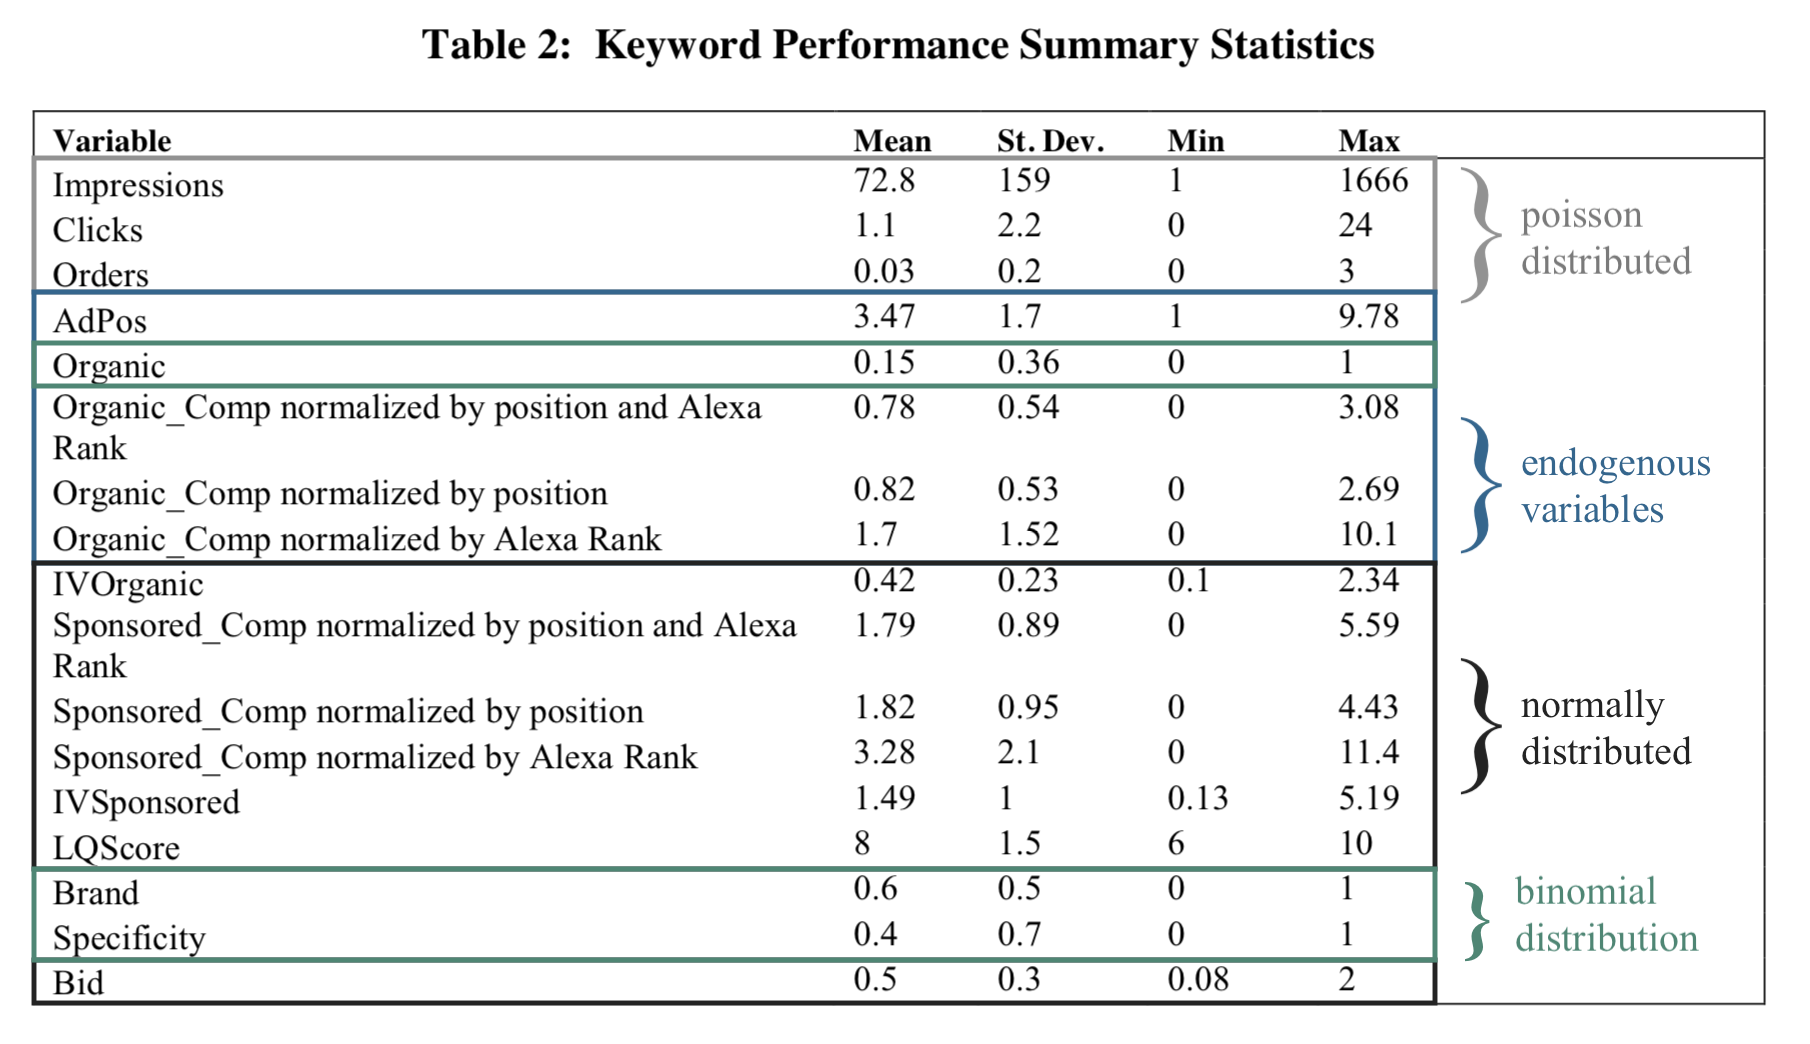
\includegraphics[scale=0.35]{Data}
    \caption{The summary statistics for the original data, including its interpreted distributions.\protect\footnotemark}
    \label{fig:Data}
\end{figure}
\footnotetext{The endogenous variables $AdPos_{kt}$ and $OrganicComp_{kt}$ were listed in this list, though contradicting the notion of "data".}

\subsection{The Distributions}
As shown in figure \ref{fig:Data}, the simulated variables follow a variety of distributions. Since the authors do not explicitly state which type of distribution each data item follows, we have assumed the most likely distribution based on the values provided in the summary statistics table. To this end, we simulated a total of 13 variables (we only focused on Sponsored Competition normalized by both position and Alexa Rank), the variable counts for each type of distribution being as follows: 
\begin{itemize}
    \item 3 Poission-distributed
    \item 3 Binomial-distributed
    \item 7 Normally distributed
\end{itemize}
The density distributions for each of these variable sets are described in figure \ref{fig:Poission}.
\subsubsection{Poisson-Distributed Variables}
\begin{figure}[!h]
    \centering
    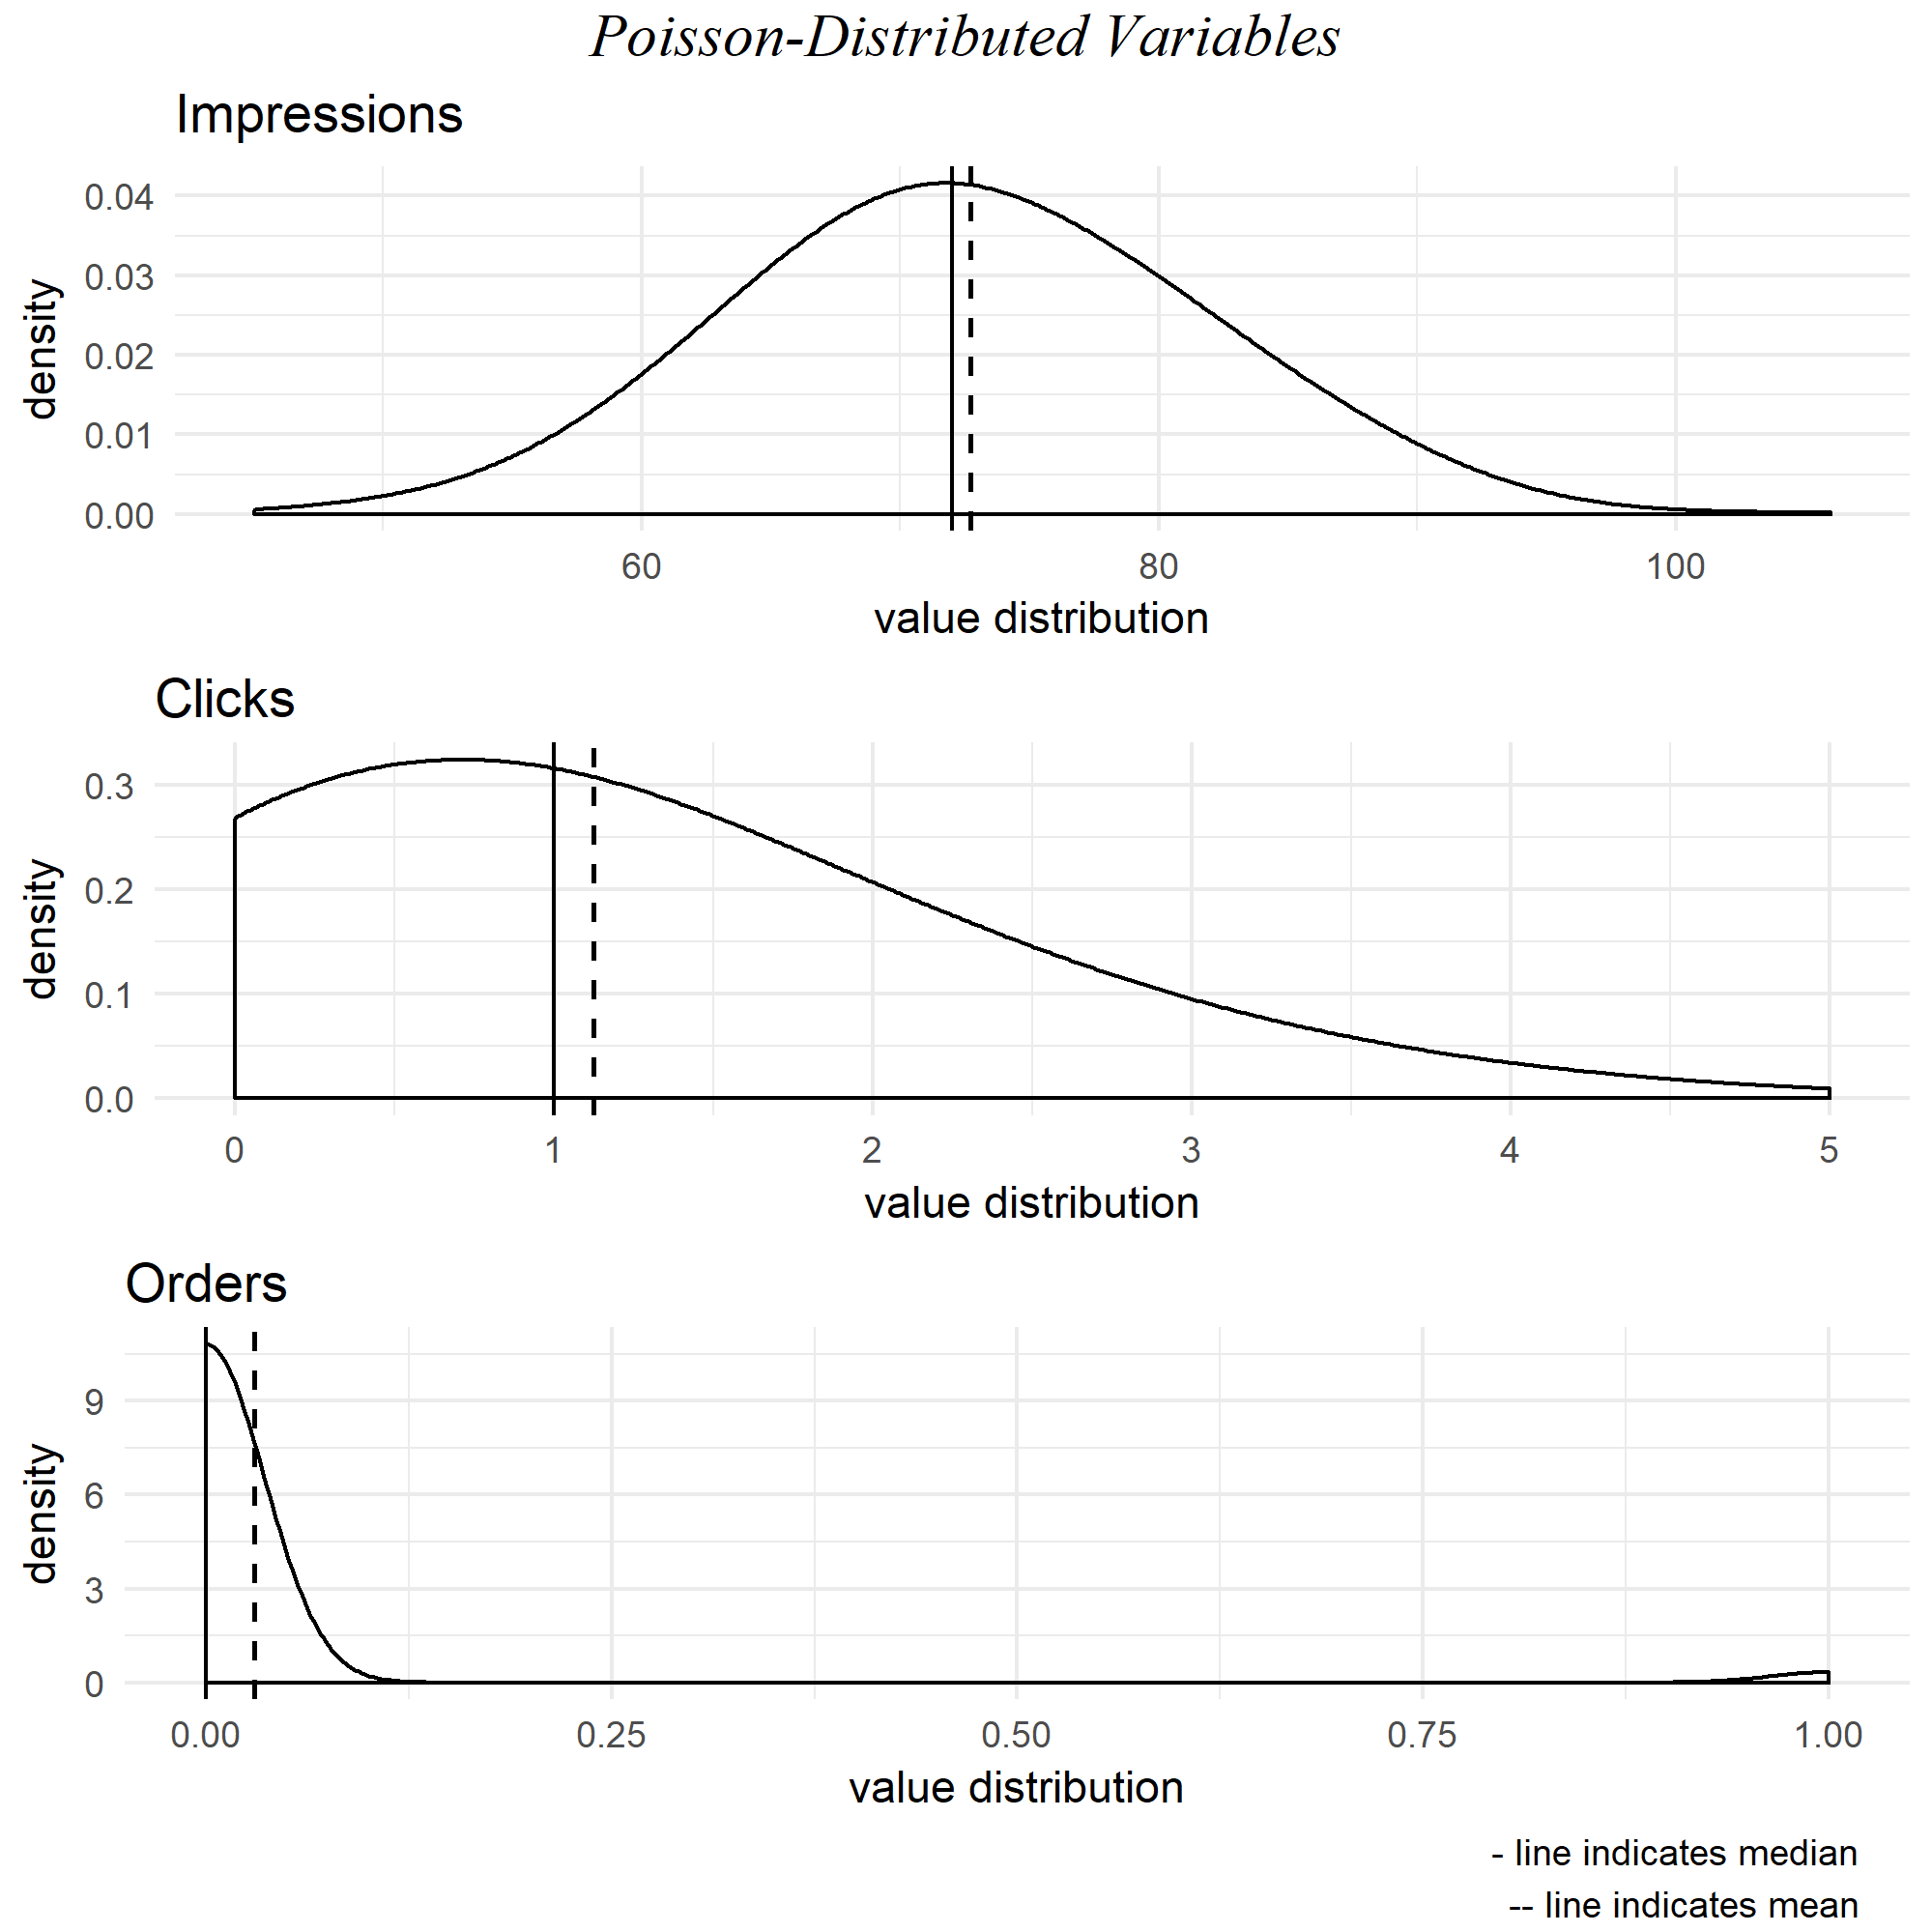
\includegraphics[scale = 0.7]{poisson_plots.png}
    \caption{Distributions for the three Poisson-distributed variables}
    \label{fig:Poission}
\end{figure}
Although it may appear to be normally distributed, the distribution for Impressions is, in fact, a Poisson distribution. To be in line with the min and max values established in the summary statistics table, any values below 1 and above 1666 (min and max, respectively), if any, have been replaced by the min and max values themselves. 
The Clicks distribution peaks close to 1 and gently slopes downward to 5, which logically makes sense as users would most often click 0 to 1 times on any particular ad in one user session. As with Impressions, Clicks has established min and max values - 0 and 24 - and any values outside of this range were replaced with the min/max values as appropriate\footnote{It is not possible, at least as far as we are aware, for a user to make -1 clicks!}.\\
Finally, the Orders distribution is bimodal, with a large peak at 0 and a much smaller peak at 1. This distribution is a bit misleading as a user can only either place an order or not, hence the 0-1 peaks. One may consider this more a binomial variable, but we chose to model it as Poisson because it is an event that occurs potentially at random and across an unknown time interval.\\
The Orders variable also has minimum- and maximum-allowed values, these being 0 and 3, respectively (as with clicks, a user cannot make a negative order).

\subsubsection{Binomial-Distributed Variables}
The three binomial variables are relatively simple in their usage, in that they represent whether an event occurred or not. Each of these variables act as a sort of on/off switch for the inclusion of the parameters in the simulation for a particular keyword at a particular time.
\begin{figure}[!h]
    \centering
    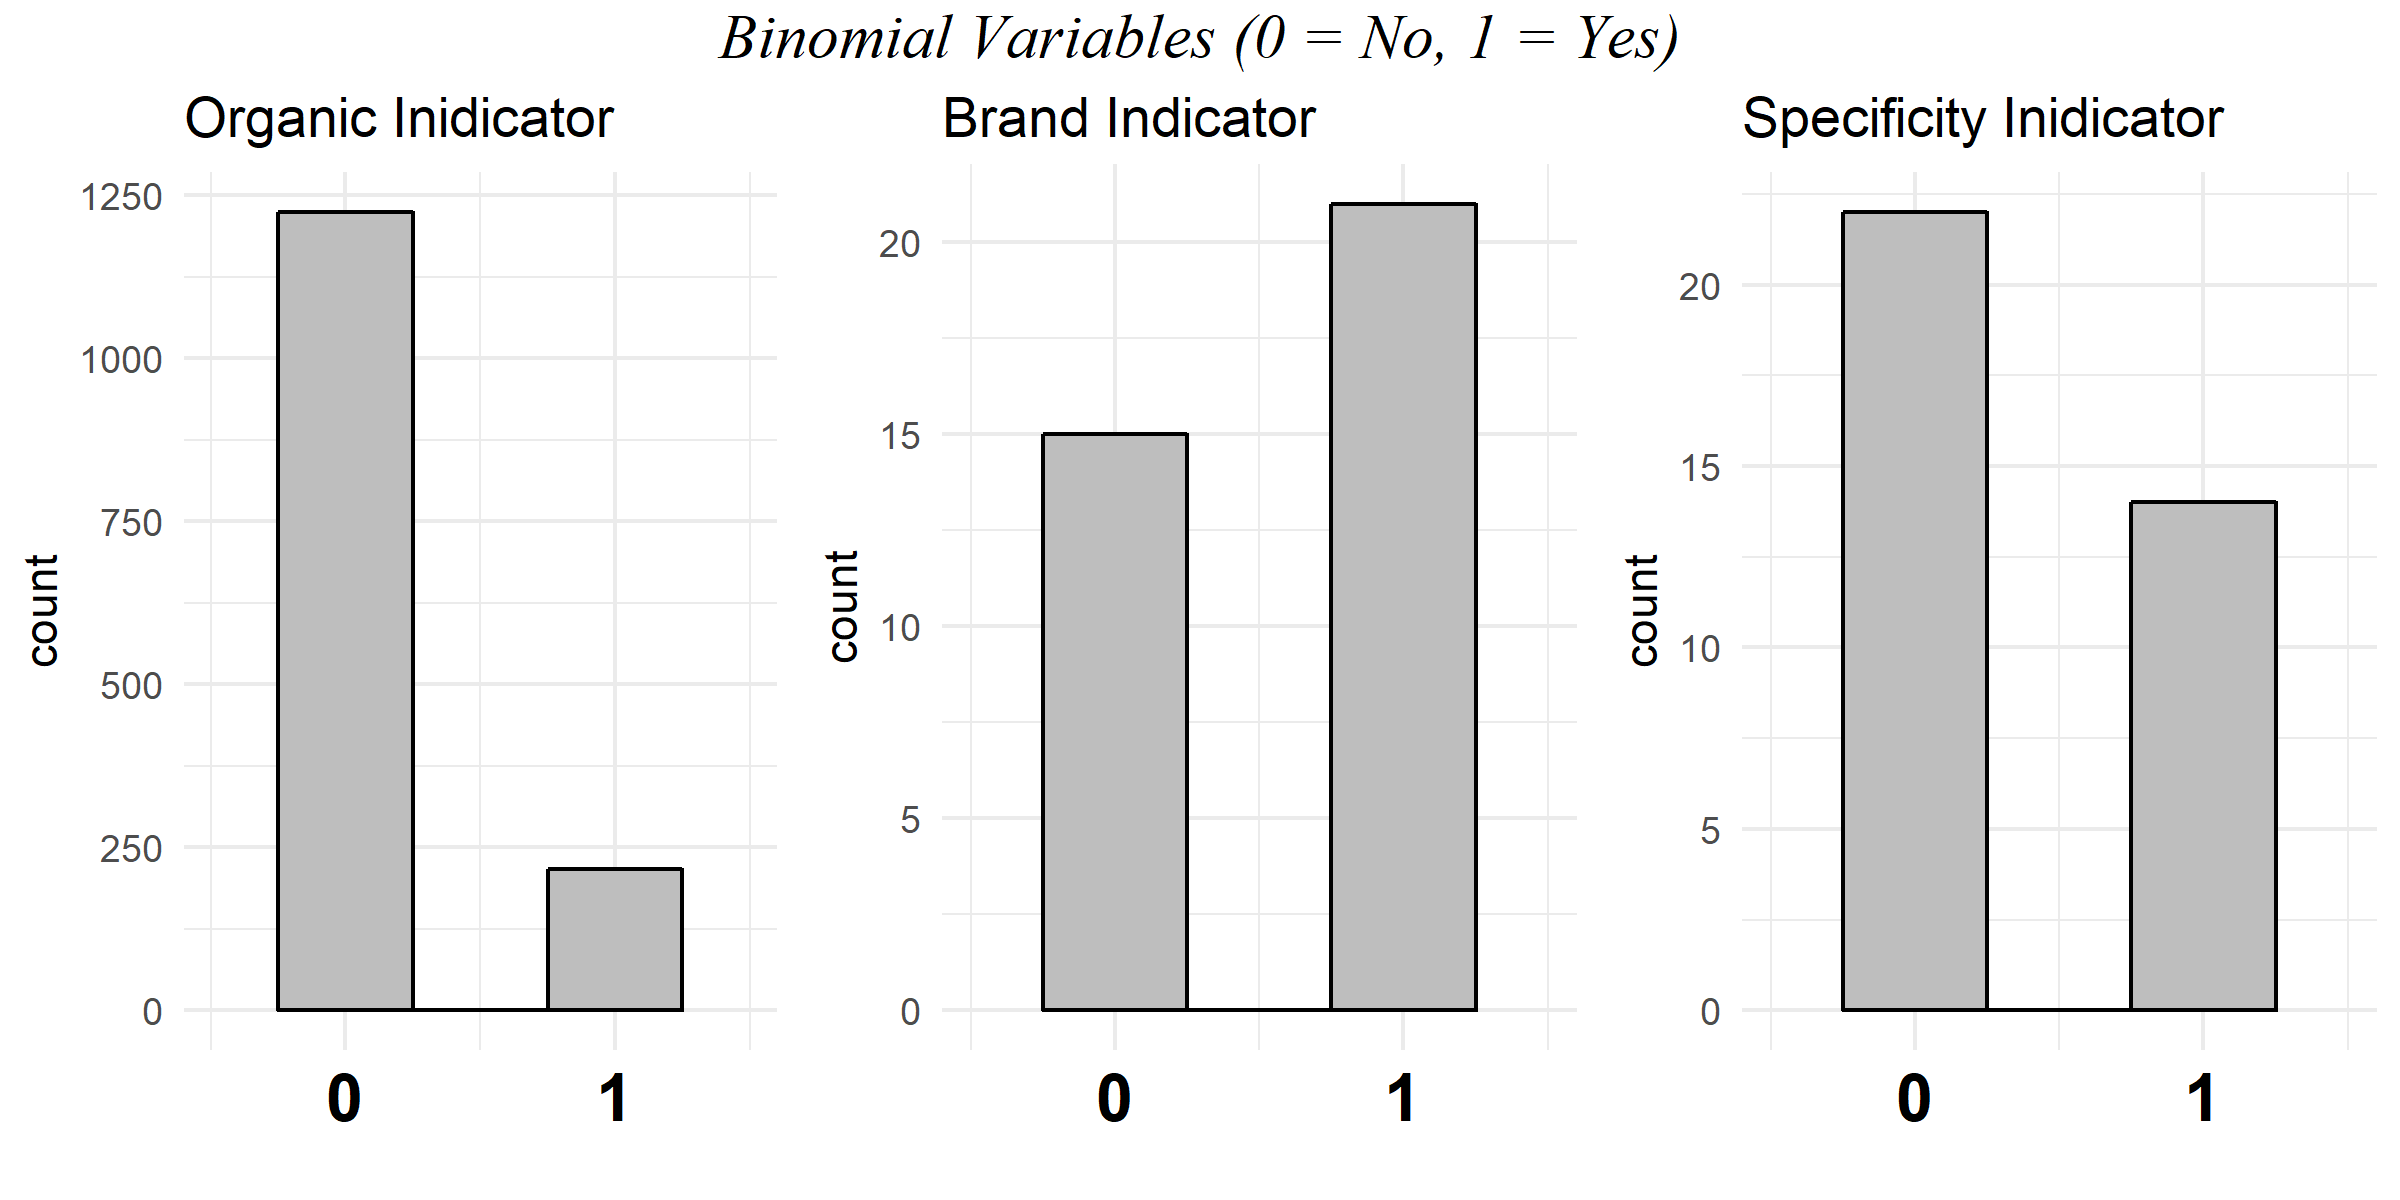
\includegraphics[scale = 0.6]{binomial_plots.png}
    \caption{Distributions for the three Binomial-distributed variables}
    \label{fig:Binomial}
\end{figure}
As mentioned in the paper, Organic is "a dummy variable which is set to one if the advertiser's organic listing appears on the first page, and is set to zero otherwise"\citep[p. 20]{agarwal_organic_2015}. Similarly, Brand is an indicator variable which is set to 1 if a known brand name is in the keyphrase used in the experiment, and is 0 if a brand name is not included.\\
Specificity is a bit more involved - this is actually an indicator of which level in the resulting website's site hierarchy the user reaches when routed through the search engine (i.e., how close to the actual searched-for product does the user get when they click on the link in the search engine?). For example, the specificity for a generic keyword - the authors mention 'pet food' - is 0, while a more specific keyword, such as 'dog food', is scored as a 1 \citep{agarwal_organic_2015}. The paper mentions the possibility for values greater than 1, but the maximum value for specificity given in the summary statistics table is 1, so we chose to model this variable as binomial.

\subsubsection{Normally Distributed Variables}
As might be expected, the predominance of our simulated variables follow a normal distribution.\\ 
\begin{figure}[!h]
    \centering
    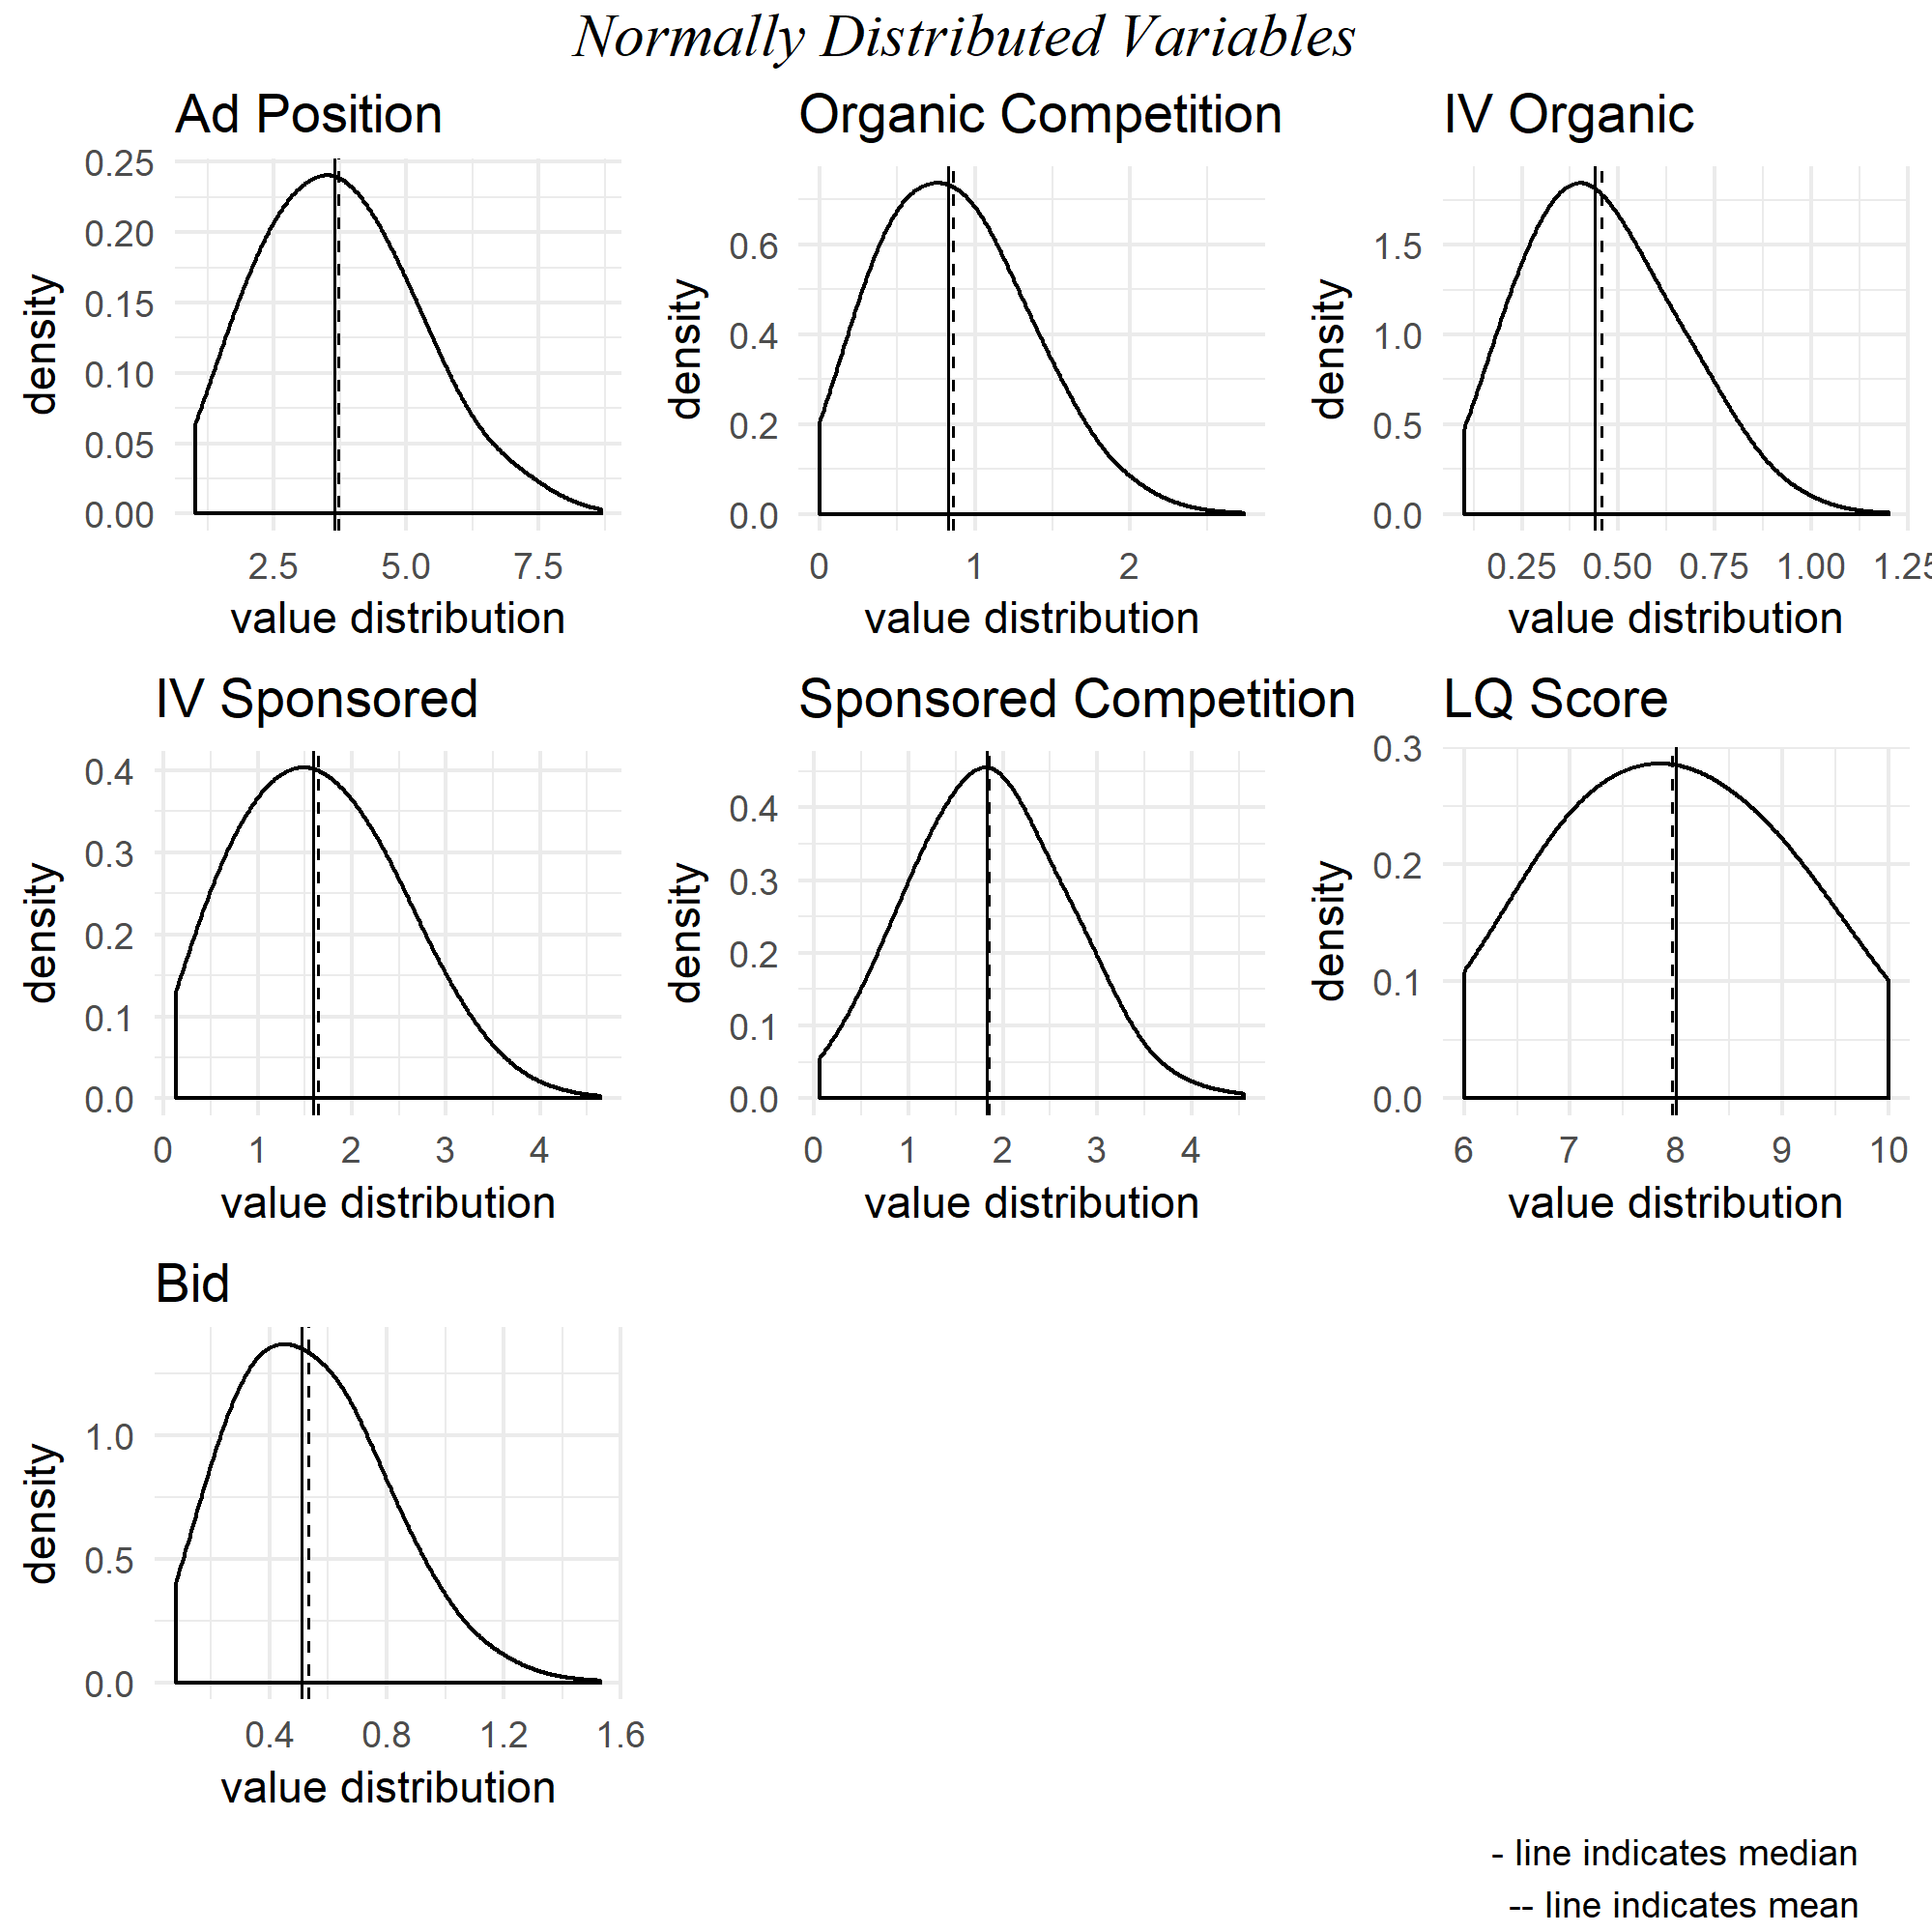
\includegraphics[scale = 0.72]{normal_plots.png}
    \caption{Distributions for the seven Normally distributed variables}
    \label{fig:Normal}
\end{figure}
It is not necessary to get into the specifics of each variable, save it to point out a few noticeable oddities about the graphs. As can be seen in figure \ref{fig:Normal}, both the mean and median are slightly right-of-center for all of the variables simulated. This is due to the fact that all of the normal distributions are \textit{truncated} normal distributions. for all but the LQ score, the minimum value given for each variable in the summary statistics table is 0; that is, the simulation would have produced values less than 0 had the minimum value in the code used not been set at 0. LQ score is even more truncated, with limits placed on its left and right tails at 6 and 10, respectively (6 being the minimum score found in the data statistics, and 10 being the maximum value allowed in the LQ scoring system).

\newpage
\subsection{Simulating the parameters of the model}
\subsubsection{The $\theta^k$s}
\begin{figure}
    \centering
    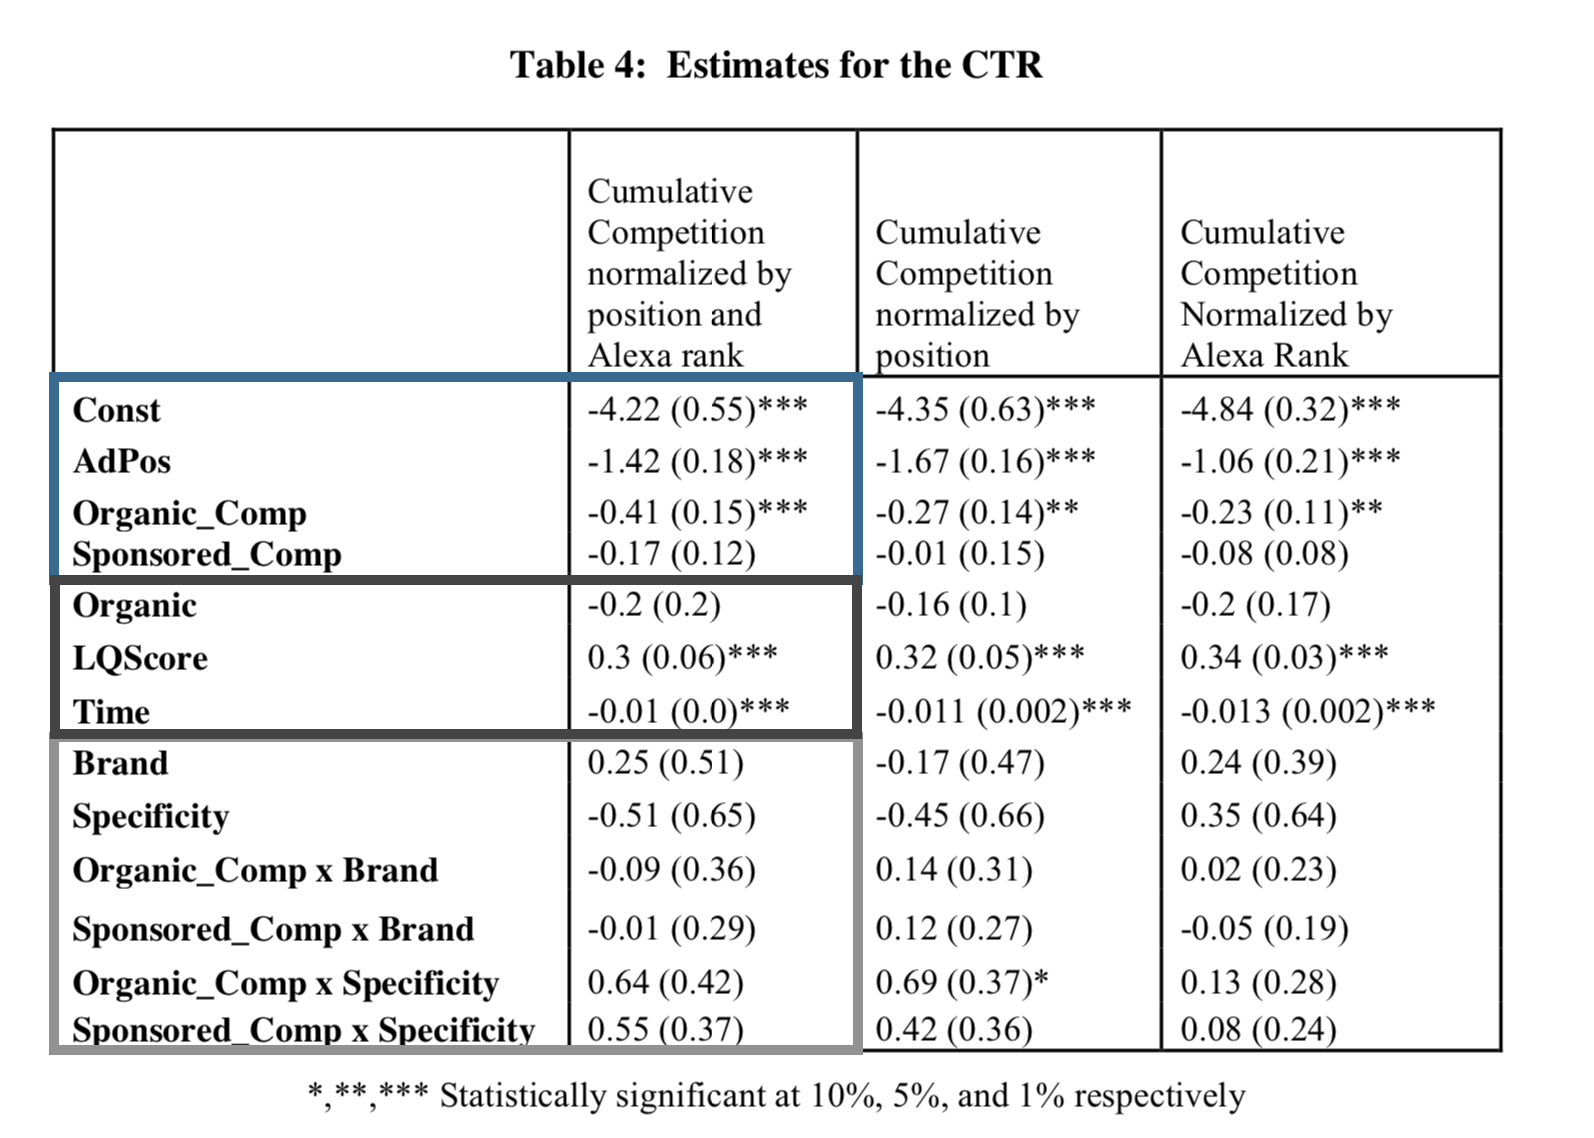
\includegraphics[scale=0.35]{table4}
    \caption{The estimates for CTR from p. 39. The authors' estimates for the $\theta^k$s in dark blue are only used for comparison. The values marked in dark grey served as constants for $\theta_4, \theta_5$ and $\theta_{Time}$. The light grey box refers to the $\Delta^{\theta}$ matrix in the code, denoted as \texttt{theta\_delta}\protect\footnotemark.}
    \label{fig:table4}
\end{figure}
\footnotetext{"Brand" and "specificity" was interpreted as $\theta_0$ x brand or specificity. As $\theta_1$,the bias for $AdPos_{kt}$, is missing it is assumed to be 0. Though $\Delta^{\theta}$ is constant for all k, the standard deviation might refer to the variation throughout the MCMC chain.}

After sampling the data, the hierarchical model's parameters needed to be estimated. Figure \ref{fig:table4} depicts how the data given was interpreted as not all values relate to a clearly identifiable part in the introduced model.\\
Essentially, the parameters from the linear model dependent on k have been drawn from a multivariate distribution with a mean $\Delta^{\theta}z_k$ specifying its relationship with the keyword specifics and a sigma matrix $V^{\theta}$. While $\Delta^{\theta}z_k$ has been taken from figure \ref{fig:table4}, $V^{\theta}$ was sampled from an Inverse Wishart distribution with 4 degrees of freedom and an identity matrix.\footnote{The matrix given in equation \ref{eq:vmatrix} is recursively defined and has thus been neglected in this section. See the estimation, section \ref{sec:estimation}, for further details.} In a sense, $V^{\theta}$ serves as a matrix for the error within the estimates of one parameter, so how the different factors come into play for the CTR. The code uses \texttt{theta\_delta} as $\Delta^{\theta}$, \texttt{VTheta} as $V^{\theta}$ and \texttt{random\_thetas} as the 4 $\theta^k$s.\\

\newpage
\begin{lstlisting}[caption={Code for simulating $\Delta^{\theta}$ and $V^{\theta}$.}]
# The theta_delta matrix is given incompletely, all missing values are treated as 0. It is all parameters depending on k in interaction with a keyword's brand and specificity, giving a 4x2 (or 2x2) matrix.
theta_delta <- matrix(c(c(0.25, -0.51), # const x brand and spec
                        c(0,0), # adpos x brand and spec
                        c(-0.09, 0.64), # organic_comp x brand and spec
                        c(-0.01,0.55)), # sponsored_comp x brand and spec
                      nrow=4, ncol=2, byrow=TRUE)
                      
# The covariance matrices: basically the error "within" a set of parameters 4 thetas depend on k, so VTheta is 4x4. All in all, there are 4 V matrices, one for each parameter set, two of size 4x4, two of size 2x2.
VTheta <- riwish(4, diag(1,nrow=4))

# Define the function to draw the parameters dependent on k
# It first simulates the u_error and then takes the delta_matrix times the z vector.
calc_coeff_matr <- function(keywords, delta_matr, z, v_matr) {
  l = matrix(nrow= 4, ncol=keywords)
  for (k in 1:keywords){
    u <- matrix(rmvnorm(n=1, mean=rep(0,nrow(delta_matr)), v_matr),
                nrow=nrow(delta_matr))
    d <- delta_matr %*% z[[k]] + u
    l[,k] <-  d
  }
  return(l)
}

# The thetas dependent on k for CTR
random_thetas <- calc_coeff_matr(num_keywords, theta_delta, z, VTheta)

# Took the mean values for the thetas that do not depend on k.
theta4 <- -0.2; theta5 <- 0.3; theta6 <- -0.01
\end{lstlisting}

\newpage
\subsubsection{The error terms $\epsilon^{\theta}_{kt}$ of the linear model}
As $V^{\theta}$ denotes the error within the different $\theta^k$s, $\Omega$ accounts for correlated error terms among $\theta$, $\beta$, $\alpha$ and $\gamma$. Based on the numbers in figure \ref{fig:errorterms}, $\Omega$ is the sigma matrix for the draw of the 4 kxt error matrices $\epsilon$ from the multivariate normal distribution, see equation \ref{eq:omega}.\\

\begin{lstlisting}[caption={Code for generating the error terms.}]
#------------calculate the error terms-------------------#
r1 <- c(0.370,	-0.036,	0.000,	-0.005)
r2 <- c(-0.036,	0.232,	0.007,	0.02)
r3 <- c(0,	0.007,	0.064,	-0.005)
r4 <- c(-0.005,	0.02,	-0.005,	0.087)

o_mat_cols <- c('CONV','CTR','Pos','Organic_comp')
omega_matrix <- matrix(c(r1, r2, r3, r4), nrow=4, ncol=4, byrow=TRUE, dimnames = list(o_mat_cols))
colnames(omega_matrix) <- o_mat_cols

error_terms <- rmvnorm(n = num_observations, sigma=omega_matrix)
errors <- vector(mode="list", length=4)
names(errors) <- c('theta_error','beta_error','gamma_error','alpha_error')
errors[[1]] <- matrix(error_terms[,1], nrow=num_keywords, ncol=num_days)
# [errors[[2]] till 4 in the same manner]

theta_error <- errors$theta_error
\end{lstlisting}
\begin{figure}[h!]
    \centering
    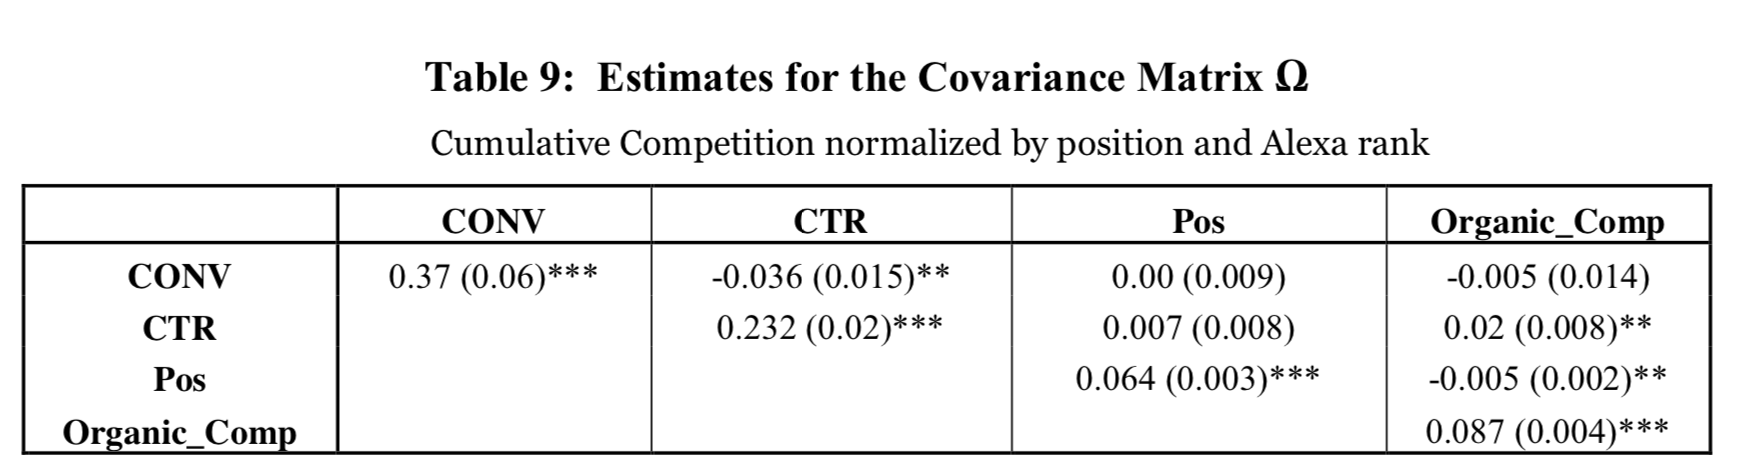
\includegraphics[scale=0.35]{errorterms}
    \caption{Table 9 from the paper, giving estimates for the error terms}
    \label{fig:errorterms}
\end{figure}

\newpage
\subsubsection{The final step towards $\Lambda^{CTR}_{kt}$}
The parameters were then combined into a linear model with the data and the error term $\epsilon^{\theta}_{kt}$, equation \ref{eq:mainlinear}. The resulting utility of clicking $U^{CTR}_{kt}$ represents the latent variable for the click-through rate. The logistic function of $U^{CTR}_{kt}$ finally leads to the dependent variable CTR, the $\Lambda^{CTR}_{kt}$ from equation \ref{eq:lambda} or \texttt{CTR\_estimate} in the code.

\begin{lstlisting}[caption={Code for simulating the parameters, shown for $\theta$.}]
# The final linear model
u_ctr <- matrix(nrow=num_keywords, ncol=num_days)
CTR_estimate <- matrix(nrow=num_keywords, ncol=num_days)
for (t in 1:num_days) {
  for (k in 1:num_keywords){
    u_ctr[k,t] <- random_thetas[[k]][1] + random_thetas[[k]][2]*adpos_eq[k,t] +
      random_thetas[[k]][3]*orgcomp_eq[k,t] + random_thetas[[k]][4]*sponsored_comp[k,t] +
      theta4*organic[k,t] + theta5*lqscore[k,t] +
      theta6*t + theta_error[k,t]
      
    CTR_estimate[k,t] <- exp(u_ctr[k,t]) / (1 + exp(u_ctr[k,t]))
    # the logit part
    }
}
# [same for betas, gammas and alphas]

\end{lstlisting}

\subsection{Simulation and Summary Statistics Comparison}
The end result of our simulation is the estimation of the CTR and CONV, ideally to be comparable to those found by the authors themselves. To compare our simulation outcome with the estimation from the paper, we first calculated the CTR and CONV based on the summary statistics given in the paper. The mean values for these are shown in table \ref{table:ctr-conv-vs}.

\begin{center}
\begin{table}[h!]
 \begin{tabular}{|c|c|c|c|c|}
 \hline
  & CTR Paper & CTR Simulation & CONV Paper & CONV Simulation \\
 \hline
 Mean & 0.01553 & 0.67544 & 0.00026 & 0.36571\\ 
 \hline
 Median & 0.01369 & 0.90372 & 0 & 0.02198 \\
 \hline
\end{tabular}
\caption{Mean and median values of simulated and paper-estimated CTR and CONV rates.}
\label{table:ctr-conv-vs}
\end{table}
\end{center}

As is apparent in \ref{table:ctr-conv-vs}, our simulation produced both CTR and CONV rate estimates with a much higher mean and median value than the summary statistics in the paper would suggest. Examining the distribution of the data helps to make the estimates we generated more understandable. 
\begin{figure}[!h]
    \centering
    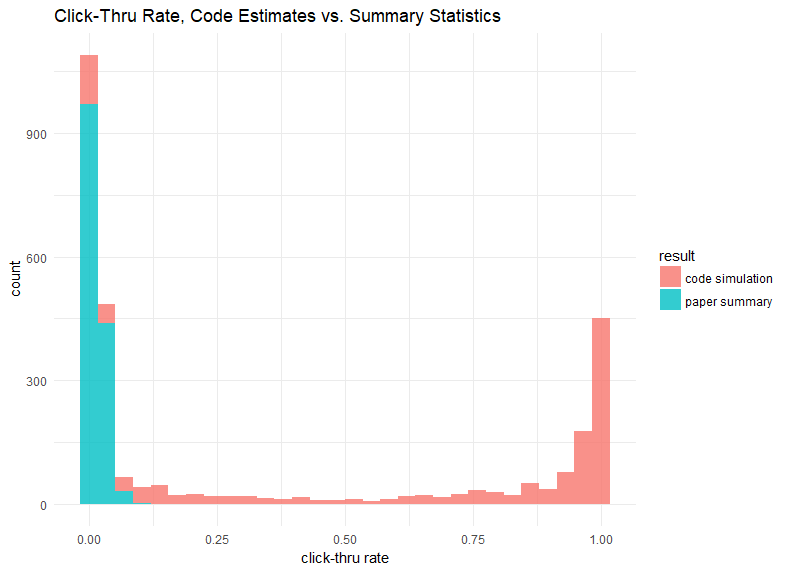
\includegraphics[scale = 0.65]{ctr_sim_code_plot.png}
    \caption{Count of simulated and summary statistic-based CTR estimates}
    \label{fig:CTR}
\end{figure}

Figure \ref{fig:CTR} shows that our simulation and the summary statistic-generated data do trend heavily toward 0, although out simulated data includes a much wider variety of possible click-through rates, as well as a great deal hovering around 1. While we did our best to follow the equations and formulas given in the paper, it is possible that we either mistakenly coded something, or that a piece of necessary information was missing in the paper itself\footnote{As mentioned, there seem to have been several noticeable omissions in the data needed to fully replicate the paper.}.

\begin{figure}[!h]
    \centering
    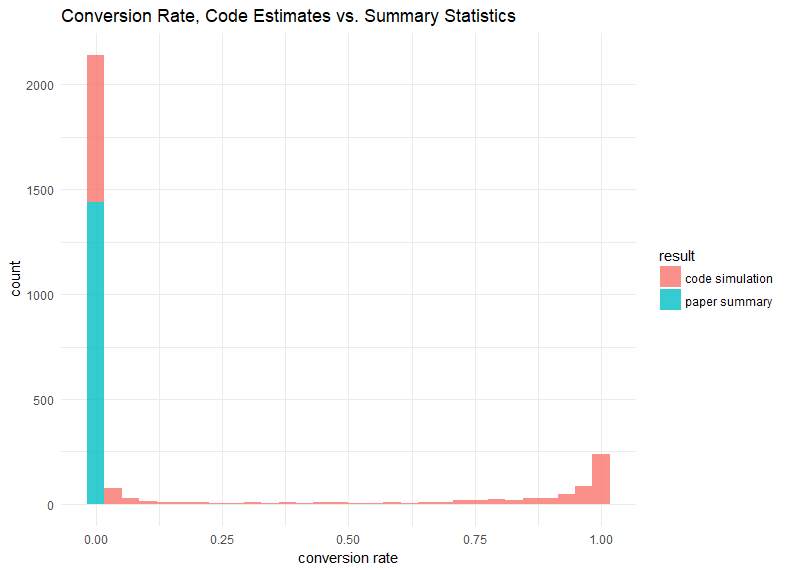
\includegraphics[scale = 0.6]{conv_sim_code_plot.png}
    \caption{Count of simulated and summary statistic-based CONV estimates}
    \label{fig:CONV}
\end{figure}

The simulated conversion rate follows a similar pattern as that of the click-through rate, as is clear in figure \ref{fig:CONV}. In keeping in line with the summary statistics data, our simulated data does trend around 0, yet, we again see a much greater distribution of data points in the simulated data. The spread does, however, seem to be less pronounced with the conversion rate than with the click-through rate.

\section{Estimating the model using a Gibbs Sampler} \label{sec:estimation}
While the simulation yields results, it used values that originally came from the Metropolis-Hastings Algorithm \citep[Appendix, p. 2]{agarwal_organic_2015}. To estimate the factors that drive the click-through rate and the orders, we implemented a Gibbs sampler. The original model runs 40,000 iterations as burn-in and 80,000 iterations in total.\\
A Bayesian model needs appropriate priors and a likelihood. The priors used in the model have been introduced as the distributions in section \ref{sec:intro}. The likelihood is a combined Bernoulli likelihood for both $U^{CTR}_{kt}$ and $U^{CONV}_{kt}$ \citep[Appendix, p. 2]{agarwal_organic_2015}. Yet, this hierarchical model is a triangular system, meaning it involves recursive elements which then become directed cycles. This imposed a problem when following the approach. The different steps have been summarized in table \ref{table:MCMC}.

\begin{longtable}{| p{0.2cm} | p{1.5cm} | p{4.5cm} | p{4.5cm} |}
    \hline
    &\textbf{Method} & \textbf{Main Focus} & \textbf{Solution}\\
    \hline \hline
    1 & JAGS & A basic implementation of the model. &\\
    &&&\\
    && The paper's likelihood is a combined likelihood for both $U^{CTR}_{kt}$ and $U^{CONV}_{kt}$ and is dependent on itself. It does not match the input required by JAGS. & It was replaced by a simple Bernoulli likelihood using \texttt{dbern()}.\\
    & & When fully specified, the model seems to be recursive, it involves directed cycles, a "simultaneous model" as also stated by the authors \citep[p. 19]{agarwal_organic_2015}. In JAGS however, directed cycles are forbidden \citep[p. 15]{JAGS}. It returned a compilation error and "possible directed cycle involving deltaTildeAlpha". The syntactically correct model \texttt{JAGS\_attempt.R} can be found in the apppendix.
    & In contrast to JAGS, BUGS allows directed cycles at a user's own risk. BUGS was therefore installed and run by \texttt{R2OpenBGUS}.\\
    \hline
    2 & BUGS & Though similar to JAGS, BUGS uses a slightly different syntax and generally offered fewer logical elements such as functions or conditional statements, e.g.: &\\
    &&&\\
    && - \texttt{\%*\%} & - matrix multiplication in loops instead of \texttt{\%*\%}\\
    && - \texttt{if} statements & - replaced \texttt{if} by \texttt{step()}\\
    && - \texttt{dbern()} throws an error & - replaced by \texttt{dnorm()} for the sake of simplicity\\
    && &\\
    \hline
    && In the end, BUGS reported a stack overflow which "can occur if there is a recursive definition of a logical node", so a simultaneous model. The syntactically correct model \texttt{BUGS\_attempt.R} can be found in the appendix. & An alternative to BUGS is the package \texttt{bayesm}. The package and the accompanying book \citep{rossibook} seem to match our model and allow for simultaneous models as well. \\
    \hline
    3 & \texttt{bayesm} & Overall, the authors seemed to have followed Rossi et al.'s approach. In particular, the function \texttt{rhierMnlRwMixture} is quite similar to the model, but would need adjustments to mirror the model. & Based on the package and its functions, an MCMC could very well be defined by us as well. After all, the Metropolis only seems to be "another algorithm".\\
    \hline
    4 & Metropolis Hastings by hand & The appended file \texttt{Metropolis\_Hastings.R} defined all necessary steps to run an MCMC by hand. It follows the appendix of the original paper. Though it encountered further dimension problems and notation issues, it was interpreted in a way that it matched dimension-wise. Unfortunately, the estimated values grow to $\infty$ after 5-7 big iterations, depending on the seed. We strongly suspect this is due to an incorrect use of the inverse, be it a notation problem or a problem in the code. See the code for more details. & To have a simple running model, JAGS was employed again.\\
    \hline
    5 & JAGS & The last JAGS model implements the main four equations from equations \ref{eq:mainlinear} and \ref{eq:endogeneous} and assumes normally distributed parameters. The $\epsilon$ error terms have been taken from the simulation in \ref{sec:simulation}. Parts of it can be seen below. The full model is denoted as \texttt{JAGS\_running.R}. & \\
    \hline
\caption{A short overview to the approaches to using a Markov Chain Monte Carlo algorithm or a Gibbs sampler for this model.}
\label{table:MCMC} 
\end{longtable}

\newpage
\begin{lstlisting}[caption={Estimating the model with a very basic JAGS version}]
modelString = "
model {
for (j in 1:N){
for (i in 1:M){

ctr[i, j] ~ dnorm(p[i,j], 1)
p[i, j] <- exp( z[i, j] ) / ( 1 + exp( z[i, j] ) )
z[i, j] <- (-4.22 + theta0) + (-1.42 + theta1) * adpos_eq[i, j] + random_thetas[3, i] * orgcomp_eq[i, j] 
+ random_thetas[4, i] * sponsored_comp[i, j] + theta4 * organic[i, j]
+ theta5 * lqscore[i, j] + theta6 * i + theta_error[i, j] 

conv[i, j] ~ dnorm(r[i, j], 1)
r[i, j] <- exp(q[i, j]) / (1 + exp(q[i, j]))
q[i,j] <- (-2.75 + beta0) + (0.81 + beta1) * adpos_eq[i, j] + random_betas[3, i] * orgcomp_eq[i, j] + 
random_betas[4, i] * sponsored_comp[i, j] + beta4 * organic[i, j] + 
beta5 * lqscore[i, j] + beta6 * i + beta_error[i, j]

adpos_eq[i, j] <- exp(random_gammas[1, i] + random_gammas[2, i] * log(bid[i, j]) + gamma2 * lqscore[i, j] +
                   gamma3 * i + gamma_error[i, j])

orgcomp_eq[i, j] <- random_alphas[1, i] + random_alphas[2, i] * iv_organic[i, j] +
                     alpha2 * i + alpha_error[i, j]

}
}
gamma2 <- -0.049
gamma3 <- -0.002

alpha2 <- -0.004

theta0 ~ dnorm(0, 0.55)
theta1 ~ dnorm(0, 0.18)
theta4 <- -0.2
theta5 <- 0.3 
theta6 <- -0.01

beta0 ~ dnorm(0, 0.68)
beta1 ~ dnorm(0, 0.28)
beta4 <- 0.17
beta5 <- -0.01
beta6 <- -0.01
}
"
writeLines( modelString, con="TEMPmodel.txt")

jags <- jags.model('TEMPmodel.txt',
                   data = list('N' = num_days,
                               'M' = num_keywords,
                               'adpos' = adpos,
                               'ctr' = CTR_estimate,
                               'conv' = CONV_estimate,
                               'bid' = bid,
                               'iv_organic' = iv_organic,
                               'orgcomp' = organic_comp,
                               'organic' = organic,
                               'sponsored_comp' = sponsored_comp,
                               'lqscore' = lqscore,
                               'theta_error' = theta_error,
                               'beta_error' = beta_error,
                               'random_betas' = random_betas,
                               'random_thetas' = random_thetas,
                               'random_gammas' = random_gammas,
                               'random_alphas' = random_alphas,
                               'gamma_error' = gamma_error,
                               'alpha_error' = alpha_error),
                   n.chains = 4,
                   n.adapt = 1000)

update(jags, 1000)

\end{lstlisting}

Although we ran into some calculation issues with our more complicated model, we were able to achieve results using a simplified version. In this version, 1000 adaptations were followed by a 1000 burn-in period. The plots here show the previous values for CTR and CONV that were calculated by our data simulation, the summary statistics-specified CTR and CONV, and the new values for these two rates calculated by JAGS.

\begin{figure}[!h]
    \centering
    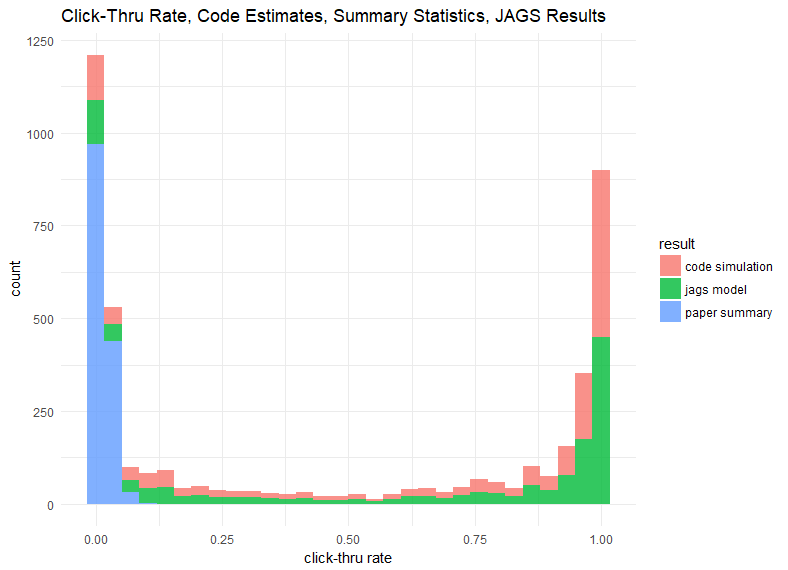
\includegraphics[scale = 0.55]{ctr_jags_plot.png}
    \caption{Count of simulated and summary statistic-based CTR estimates}
    \label{fig:ctr-jags}
\end{figure}

 The distribution of the JAGS-generated CTR values is shown as somewhere between the data-simulated values and those from the summary statistics - this is displayed in figure \ref{fig:conv-jags}. As seen in figure \ref{fig:ctr-jags}, the spread of the conversation rates also follows this pattern.

\begin{figure}[!h]
    \centering
    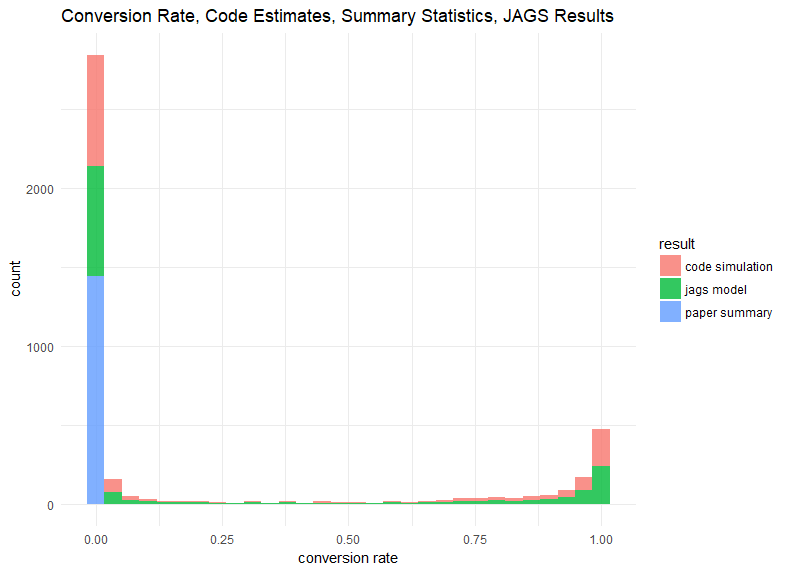
\includegraphics[scale = 0.55]{conv_jags_plot.png}
    \caption{Count of simulated and summary statistic-based CTR estimates}
    \label{fig:conv-jags}
\end{figure}

As we see in the the trace plots of theta0 and theta1 (figure \ref{fig:trace-theta0}), the distribution of the chain is relatively normal and the trajectory is stable over time. As we are expecting to see normal distributions, this is a good indicator that things are working properly \citep{MCMCDiagnostic}.

\begin{figure}[!h]
    \centering
    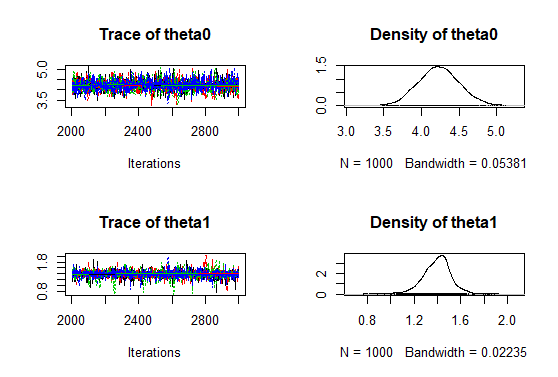
\includegraphics[scale = 0.65]{theta0_trace.png}
    \caption{Trace plot of Theta0 and Theta1 from JAGS model}
    \label{fig:trace-theta0}
\end{figure}

Looking at figure \ref{fig:gelman-theta0}, the Gelman plots for theta0 and theta1, we see that the appear to be well-disbursed throughout the sampling period. This indicates that our chains are relatively similar to each other, at least in terms of values for theta0.

\begin{figure}[!h]
    \centering
    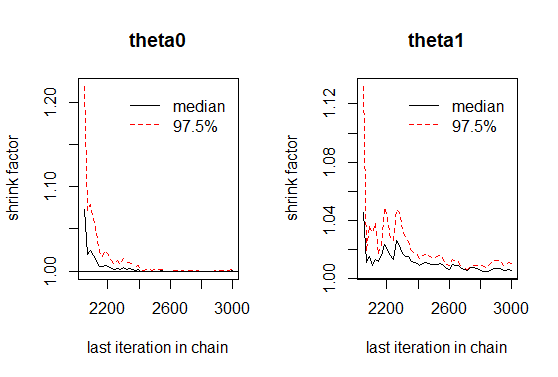
\includegraphics[scale = 0.65]{theta0_gelman.png}
    \caption{Gelman plots of Theta0 and Theta1}
    \label{fig:gelman-theta0}
\end{figure}
\section{Evaluation of the model}
\comm{Main content:
- Are the estimates by the authors realistic?
- reliability: would we be able to replicate the model with newer data? Would the construction of the model still work or is it a one-time-only model that only works with the data from 2009?
- what to enhance in the paper?
- convergence of the model? what do the plots say?}
The model involves a number of short-comings regarding its notation and mathematical formulation, and many errors have been reported above. In general, following the verified approach by Rossi et al. should ensure a conclusive model. From a mathematical perspective, the chosen levels of hierarchy, the way to account for endogeneity and the chosen logit function make sense despite the level of complexity. The simultaneity however adds a certain fragility to the method, the numbers, and thus the reliability of the instrument as a whole. This system cannot be easily reproduced nor can the correctness of the results be cross-validated.\\
Furthermore, some parameters, such as data on competitors, are completely missing. This forced us to focus on each particular detail of the model and effectively interpret the missing data in the most probable way according to our interpretation. While this is the only approach we could have taken given the scarcity of the data, it made us question the accurateness of the estimations and whether the results can still hold.\\
Another thing worth mentioning is that the model described in the paper cannot be replicated entirely due to a different layout of Google search pages. The positioning of both organic and paid ads has changed a great deal since 2009 (when the experiment in the Agarwal et al. paper was conducted), which also means that the way users interact with the ads would not be the same today. Examples of ad positions then and now are provided below: Figure \ref{fig:Google2009} from 2009 is taken from the paper itself, while the current one in Figure \ref{fig:Googletoday} is prepared by the group.\\

\begin{figure}
    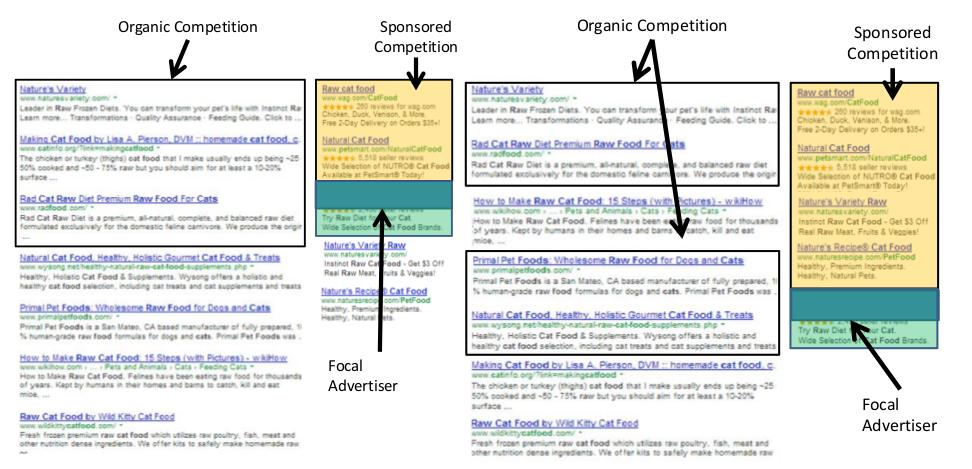
\includegraphics[scale=0.35]{organic_vs_sponsored.jpeg}
    \caption{Google ad positions in 2009}
    \label{fig:Google2009}
\end{figure}

\begin{figure}
    \centering
    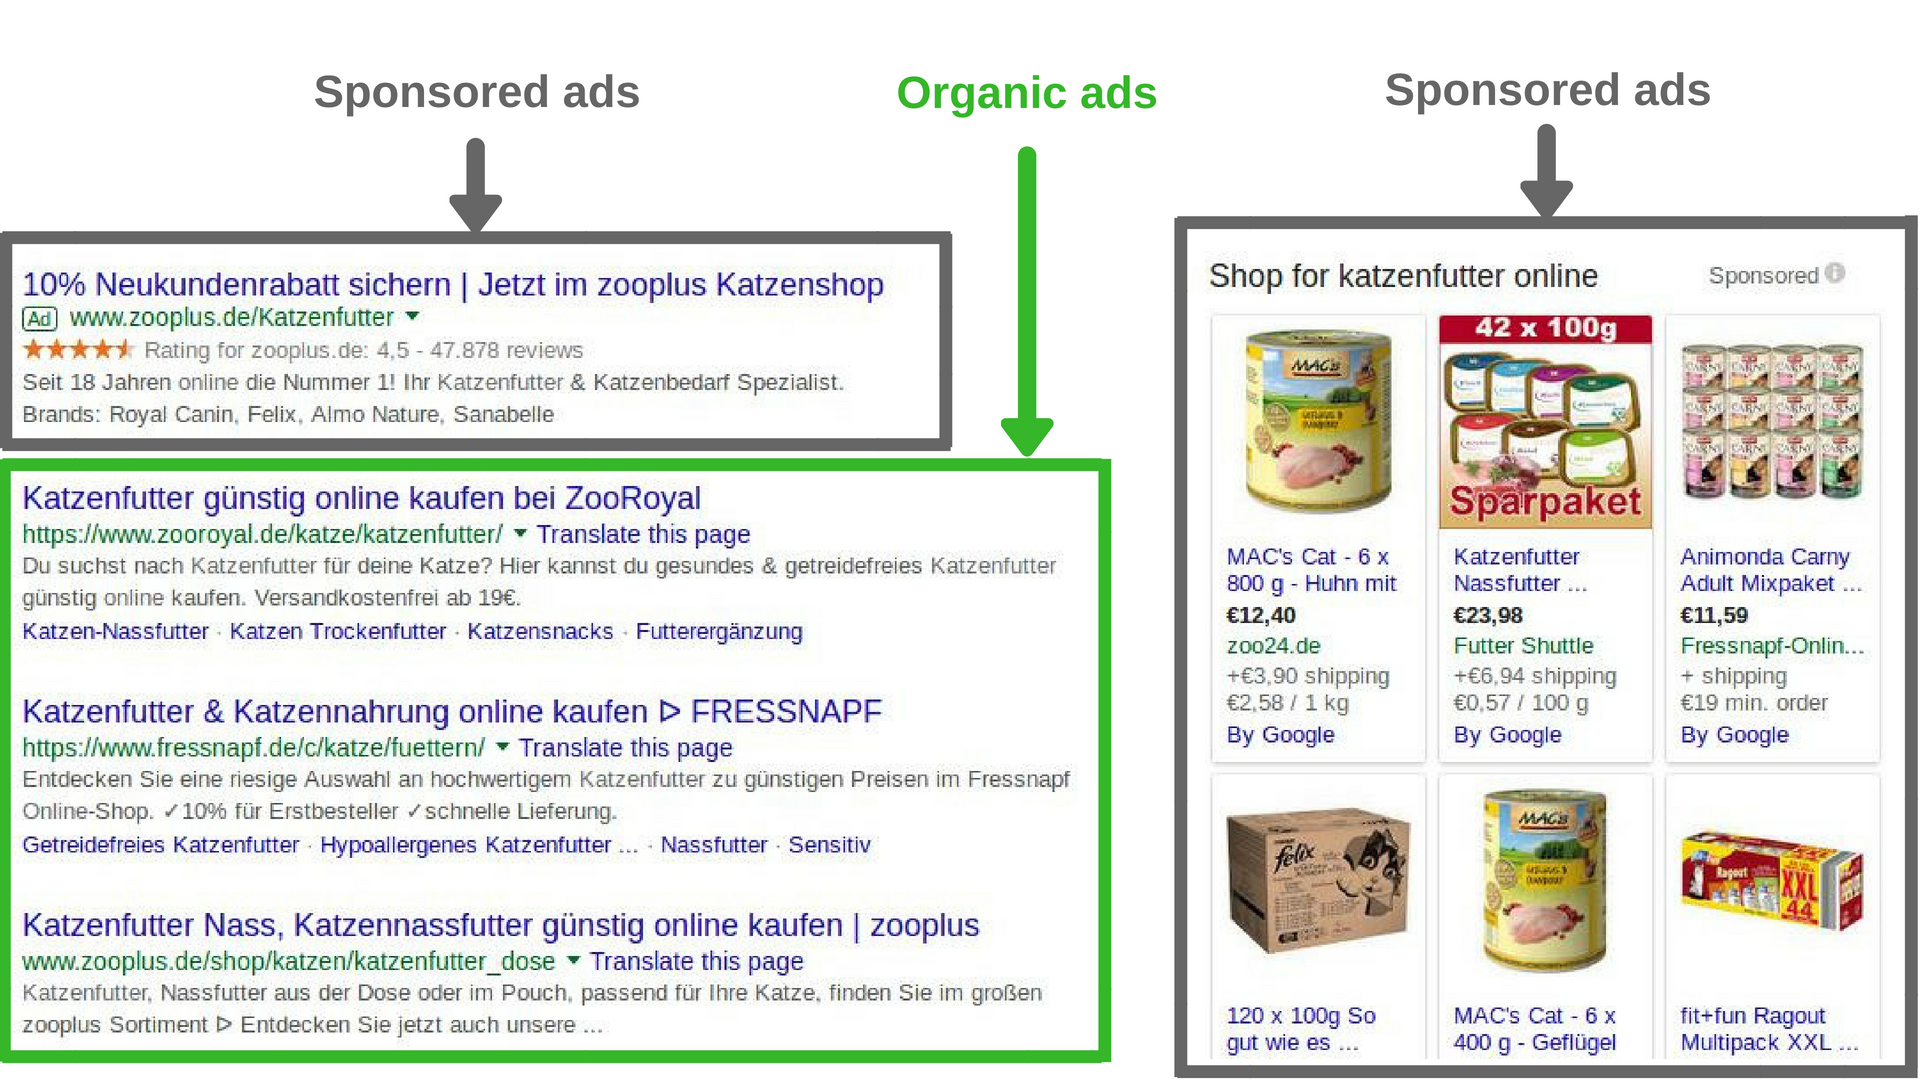
\includegraphics[scale=0.2]{catfoodsearch.png} 
    \caption{Google ad positions today}
    \label{fig:Googletoday}
\end{figure}

\newpage
All in all, the model by Agarwal et al. posed quite a few challenges when trying to follow the approach. The model as such, and especially its documentation, could be improved in the future. We would like to close this paper with a small statement: if pet food were a problem, then the most simple solution might be the correct one, according to William of Ockham. Just give the dogs some petfood.

\begin{center}
    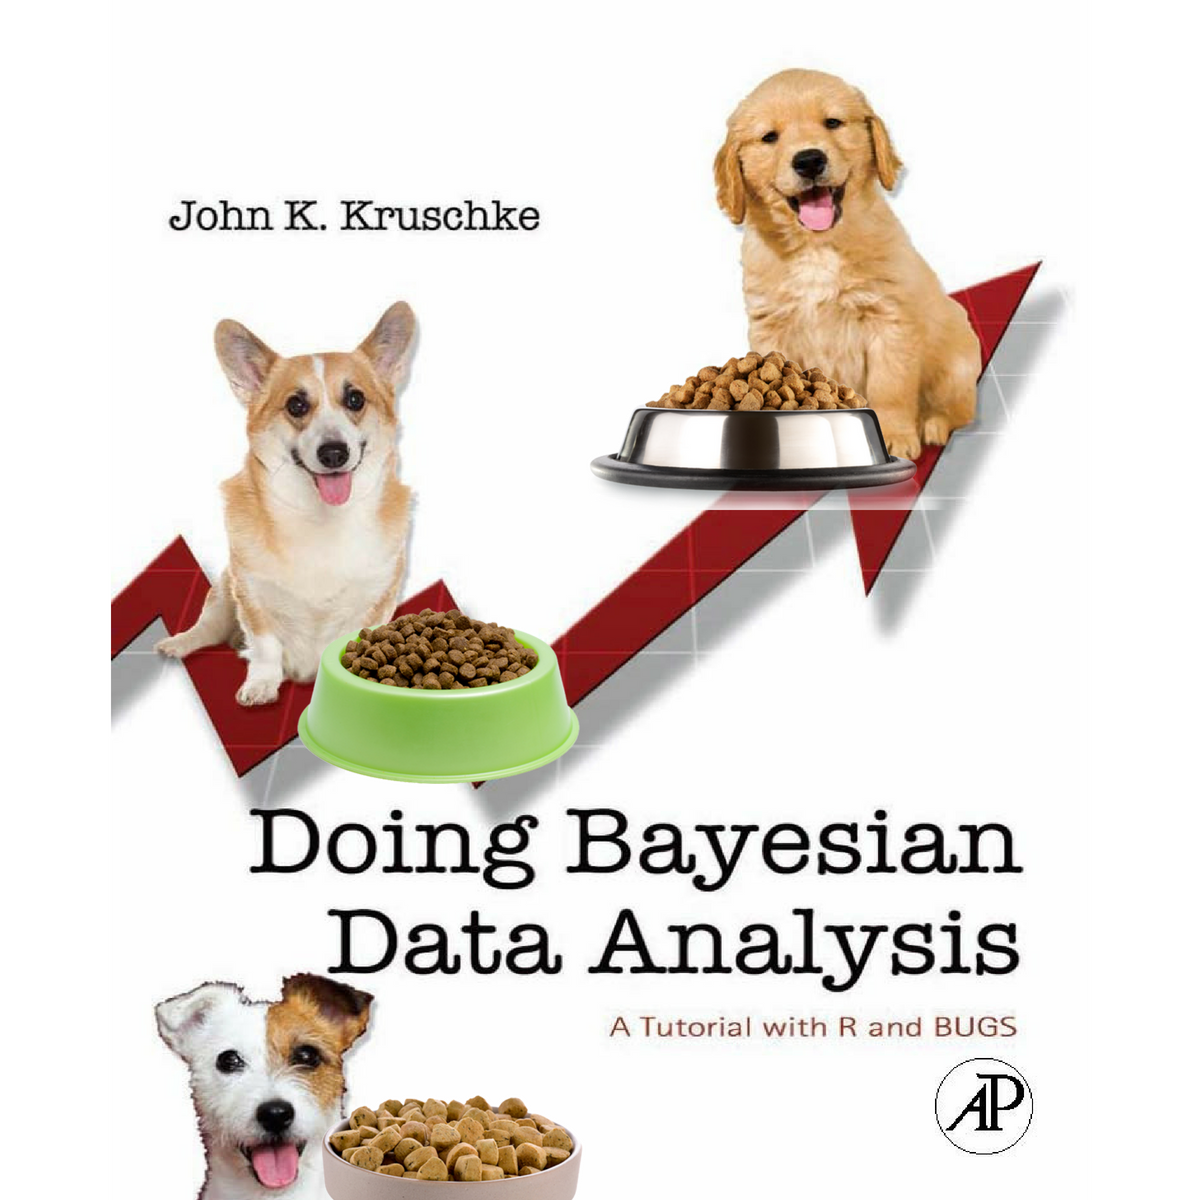
\includegraphics[scale=0.28]{outro.png}
\end{center}

\bibliographystyle{apalike}
\bibliography{references}

%\section{Appendix}
\subsection*{Code to generate the data}

\lstinputlisting[caption={The full code for generating the data and reconstructing the model.}]{Agarwalmodel.R} %just upload the R file and call it Agarwalmodel.r


\subsection{Code to simulate the MCMC}
%\lstinputlisting[caption={The full code for running the MCMC simulation using JAGS.}]{AgarwalJAGS.R} %just upload the R file and call it AgarwalJAGS.r
\section{Eidesstattliche Erklärung}
Hiermit versichere ich, dass die Arbeit selbständig verfasst und keine anderen als die angegebenen Quellen und Hilfsmittel benutzt wurden, alle Stellen der Arbeit, die wortwörtlich oder sinngemäß aus anderen Quellen übernommen und als solche kenntlich gemacht wurden und die Arbeit in gleicher oder ähnlicher Form noch keiner Prüfungsbehörde vorgelegt wurde.\\[10pt]

\noindent
\begin{tabular}{lcl}
    \rule{5cm}{0.5pt}\\
    Datum und Unterschrift
\end{tabular}
\vspace{0.5cm}

\noindent
\begin{tabular}{lcl}
    \rule{5cm}{0.5pt}\\
    Datum und Unterschrift\\
\end{tabular}
\vspace{0.5cm}

\noindent
\begin{tabular}{lcl}
    \rule{5cm}{0.5pt}\\
    Datum und Unterschrift\\
\end{tabular}
\vspace{1cm}

\noindent
\Large
\textbf{Statutory Declaration}\\[10pt]
\normalsize
I hereby declare that I have authored this thesis independently, that I have not used other than the declared sources / resources, and that I have explicitly marked all material which has been quoted either literally or by content from the used sources.\\[10pt]

\noindent
\begin{tabular}{l}
    \rule{5cm}{0.5pt}\\
    Date and signature\\
\end{tabular}
\vspace{0.5cm}

\noindent
\begin{tabular}{l}
    \rule{5cm}{0.5pt}\\
    Date and signature\\
\end{tabular}
\vspace{0.5cm}

\noindent
\begin{tabular}{l}
    \rule{5cm}{0.5pt}\\
    Date and signature\\
\end{tabular}

\end{document}

Imported from Another project/00\_main.tex, at 10:44 pm Today
 
